% Options for packages loaded elsewhere
\PassOptionsToPackage{unicode}{hyperref}
\PassOptionsToPackage{hyphens}{url}
%
\documentclass[
]{article}
\usepackage{amsmath,amssymb}
\usepackage{iftex}
\ifPDFTeX
  \usepackage[T1]{fontenc}
  \usepackage[utf8]{inputenc}
  \usepackage{textcomp} % provide euro and other symbols
\else % if luatex or xetex
  \usepackage{unicode-math} % this also loads fontspec
  \defaultfontfeatures{Scale=MatchLowercase}
  \defaultfontfeatures[\rmfamily]{Ligatures=TeX,Scale=1}
\fi
\usepackage{lmodern}
\ifPDFTeX\else
  % xetex/luatex font selection
\fi
% Use upquote if available, for straight quotes in verbatim environments
\IfFileExists{upquote.sty}{\usepackage{upquote}}{}
\IfFileExists{microtype.sty}{% use microtype if available
  \usepackage[]{microtype}
  \UseMicrotypeSet[protrusion]{basicmath} % disable protrusion for tt fonts
}{}
\makeatletter
\@ifundefined{KOMAClassName}{% if non-KOMA class
  \IfFileExists{parskip.sty}{%
    \usepackage{parskip}
  }{% else
    \setlength{\parindent}{0pt}
    \setlength{\parskip}{6pt plus 2pt minus 1pt}}
}{% if KOMA class
  \KOMAoptions{parskip=half}}
\makeatother
\usepackage{xcolor}
\usepackage[margin=1in]{geometry}
\usepackage{graphicx}
\makeatletter
\newsavebox\pandoc@box
\newcommand*\pandocbounded[1]{% scales image to fit in text height/width
  \sbox\pandoc@box{#1}%
  \Gscale@div\@tempa{\textheight}{\dimexpr\ht\pandoc@box+\dp\pandoc@box\relax}%
  \Gscale@div\@tempb{\linewidth}{\wd\pandoc@box}%
  \ifdim\@tempb\p@<\@tempa\p@\let\@tempa\@tempb\fi% select the smaller of both
  \ifdim\@tempa\p@<\p@\scalebox{\@tempa}{\usebox\pandoc@box}%
  \else\usebox{\pandoc@box}%
  \fi%
}
% Set default figure placement to htbp
\def\fps@figure{htbp}
\makeatother
\setlength{\emergencystretch}{3em} % prevent overfull lines
\providecommand{\tightlist}{%
  \setlength{\itemsep}{0pt}\setlength{\parskip}{0pt}}
\setcounter{secnumdepth}{-\maxdimen} % remove section numbering
\ifLuaTeX
\usepackage[bidi=basic]{babel}
\else
\usepackage[bidi=default]{babel}
\fi
\babelprovide[main,import]{french}
% get rid of language-specific shorthands (see #6817):
\let\LanguageShortHands\languageshorthands
\def\languageshorthands#1{}
\usepackage{bookmark}
\IfFileExists{xurl.sty}{\usepackage{xurl}}{} % add URL line breaks if available
\urlstyle{same}
\hypersetup{
  pdftitle={Les demandeurs d'emploi inscrits à Pôle Emploi},
  pdfauthor={@statjunior},
  pdflang={fr-FR},
  hidelinks,
  pdfcreator={LaTeX via pandoc}}

\title{Les demandeurs d'emploi inscrits à Pôle Emploi}
\usepackage{etoolbox}
\makeatletter
\providecommand{\subtitle}[1]{% add subtitle to \maketitle
  \apptocmd{\@title}{\par {\large #1 \par}}{}{}
}
\makeatother
\subtitle{Données administratives du 2e trimestre 2024.}
\author{@statjunior}
\date{25 juillet 2024}

\begin{document}
\maketitle

\section{Présentation}\label{pruxe9sentation}

Ce rapport \emph{RMarkdown} analyse les effectifs de demandeurs d'emploi
à Pôle Emploi au 2ème trimestre 2024. Les données sont produites par la
Dares et Pôle Emploi à partir de sources administratives exhaustives.

\textbf{Les données sur les demandeurs d'emploi de Pôle Emploi ne
doivent pas être confondues avec celles sur le chômage au sens du BIT
produites par l'Insee}. Un autre rapport (consultable
\href{https://github.com/statjunior/Statjunior/tree/main/March\%C3\%A9\%20du\%20travail\%20et\%20ch\%C3\%B4mage/Ch\%C3\%B4mage\%20BIT\%2C\%20halo\%20et\%20sous\%20emploi\%20-\%20Enqu\%C3\%AAte\%20Emploi/}{en
cliquant ici}) analyse les différents indicateurs du chômage au sens de
l'Insee.

Dans un premier temps, le rapport présente le nombre de demandeurs
d'emploi inscrits à Pôle Emploi par catégorie. Les catégorie A-B-C
regroupent les inscrits tenus de chercher un emploi, alors que les
catégories D et E regroupent les inscrits dispensés de recherche
d'emploi. La catégorie A inclut uniquement les inscrits sans emploi,
alors que les catégories B et C regroupent les inscrits en emploi à
temps partiel (inférieur à 78 heures par mois pour la catégorie B,
supérieur à 78 heures par mois pour la catégorie C).

On s'intéresse ensuite à la structure des inscrits à Pôle Emploi,
d'abord par sexe puis par tranches d'âge.

On relève également la durée d'inscription à Pôle Emploi, décomposée
ensuite par tranches d'âge ou bien entre inscrits et sortants.

On analyse enfin les motifs d'entrée et de sortie à Pôle Emploi au cours
du 2ème trimestre 2024. Une attention particulière doit être portée à
l'évolution des radiations ou du non renouvellement d'inscription, dans
la mesure où il s'agit de sources administratives. Les comportements
d'inscription et de contrôle administratif expliquent en effet une
partie des variations, parallèlement à la conjoncture du marché du
travail. On présente aussi la part des inscrits indemnisés par Pôle
Emploi.

Le rapport se conclut avec une confrontation des différentes sources des
demandeurs d'emploi, à savoir les données administratives de Pôle Emploi
présentées dans ce rapport avec les données d'enquête de l'Insee
(mesurant le chômage BIT). On présente pour chaque trimestre l'écart
entre le nombre de catégories A à Pôle Emploi et le nombre de chômeurs
BIT mesurés par l'Insee.

Ce rapport a été compilé automatiquement avec le logiciel \texttt{R}, le
25 juillet 2024 à 13 heures et 47 minutes. Les potentielles erreurs
présentes dans ce document relèvent uniquement de la responsabilité de
Statjunior.

Le code source permettant de générer ce document est disponible sur Git
\href{https://github.com/statjunior/Statjunior/tree/main/Demandeurs\%20d'emploi\%20(Pole\%20Emploi)/}{en
cliquant ici}.

\newpage

\section{Inscriptions à Pôle Emploi par
catégories}\label{inscriptions-uxe0-puxf4le-emploi-par-catuxe9gories}

\subsection{Catégorie A, Catégorie A-B-C et toutes catégories (France
hors
Mayotte)}\label{catuxe9gorie-a-catuxe9gorie-a-b-c-et-toutes-catuxe9gories-france-hors-mayotte}

Au 2ème trimestre 2024, le nombre de demandeurs d'emploi en catégorie A
s'établit à 3 millions d'individus.

Il y a 5.4 millions d'individus en catégories A, B ou C et 6.1 millions
d'individus inscrits à Pôle Emploi en comptant toutes les catégories.

\pandocbounded{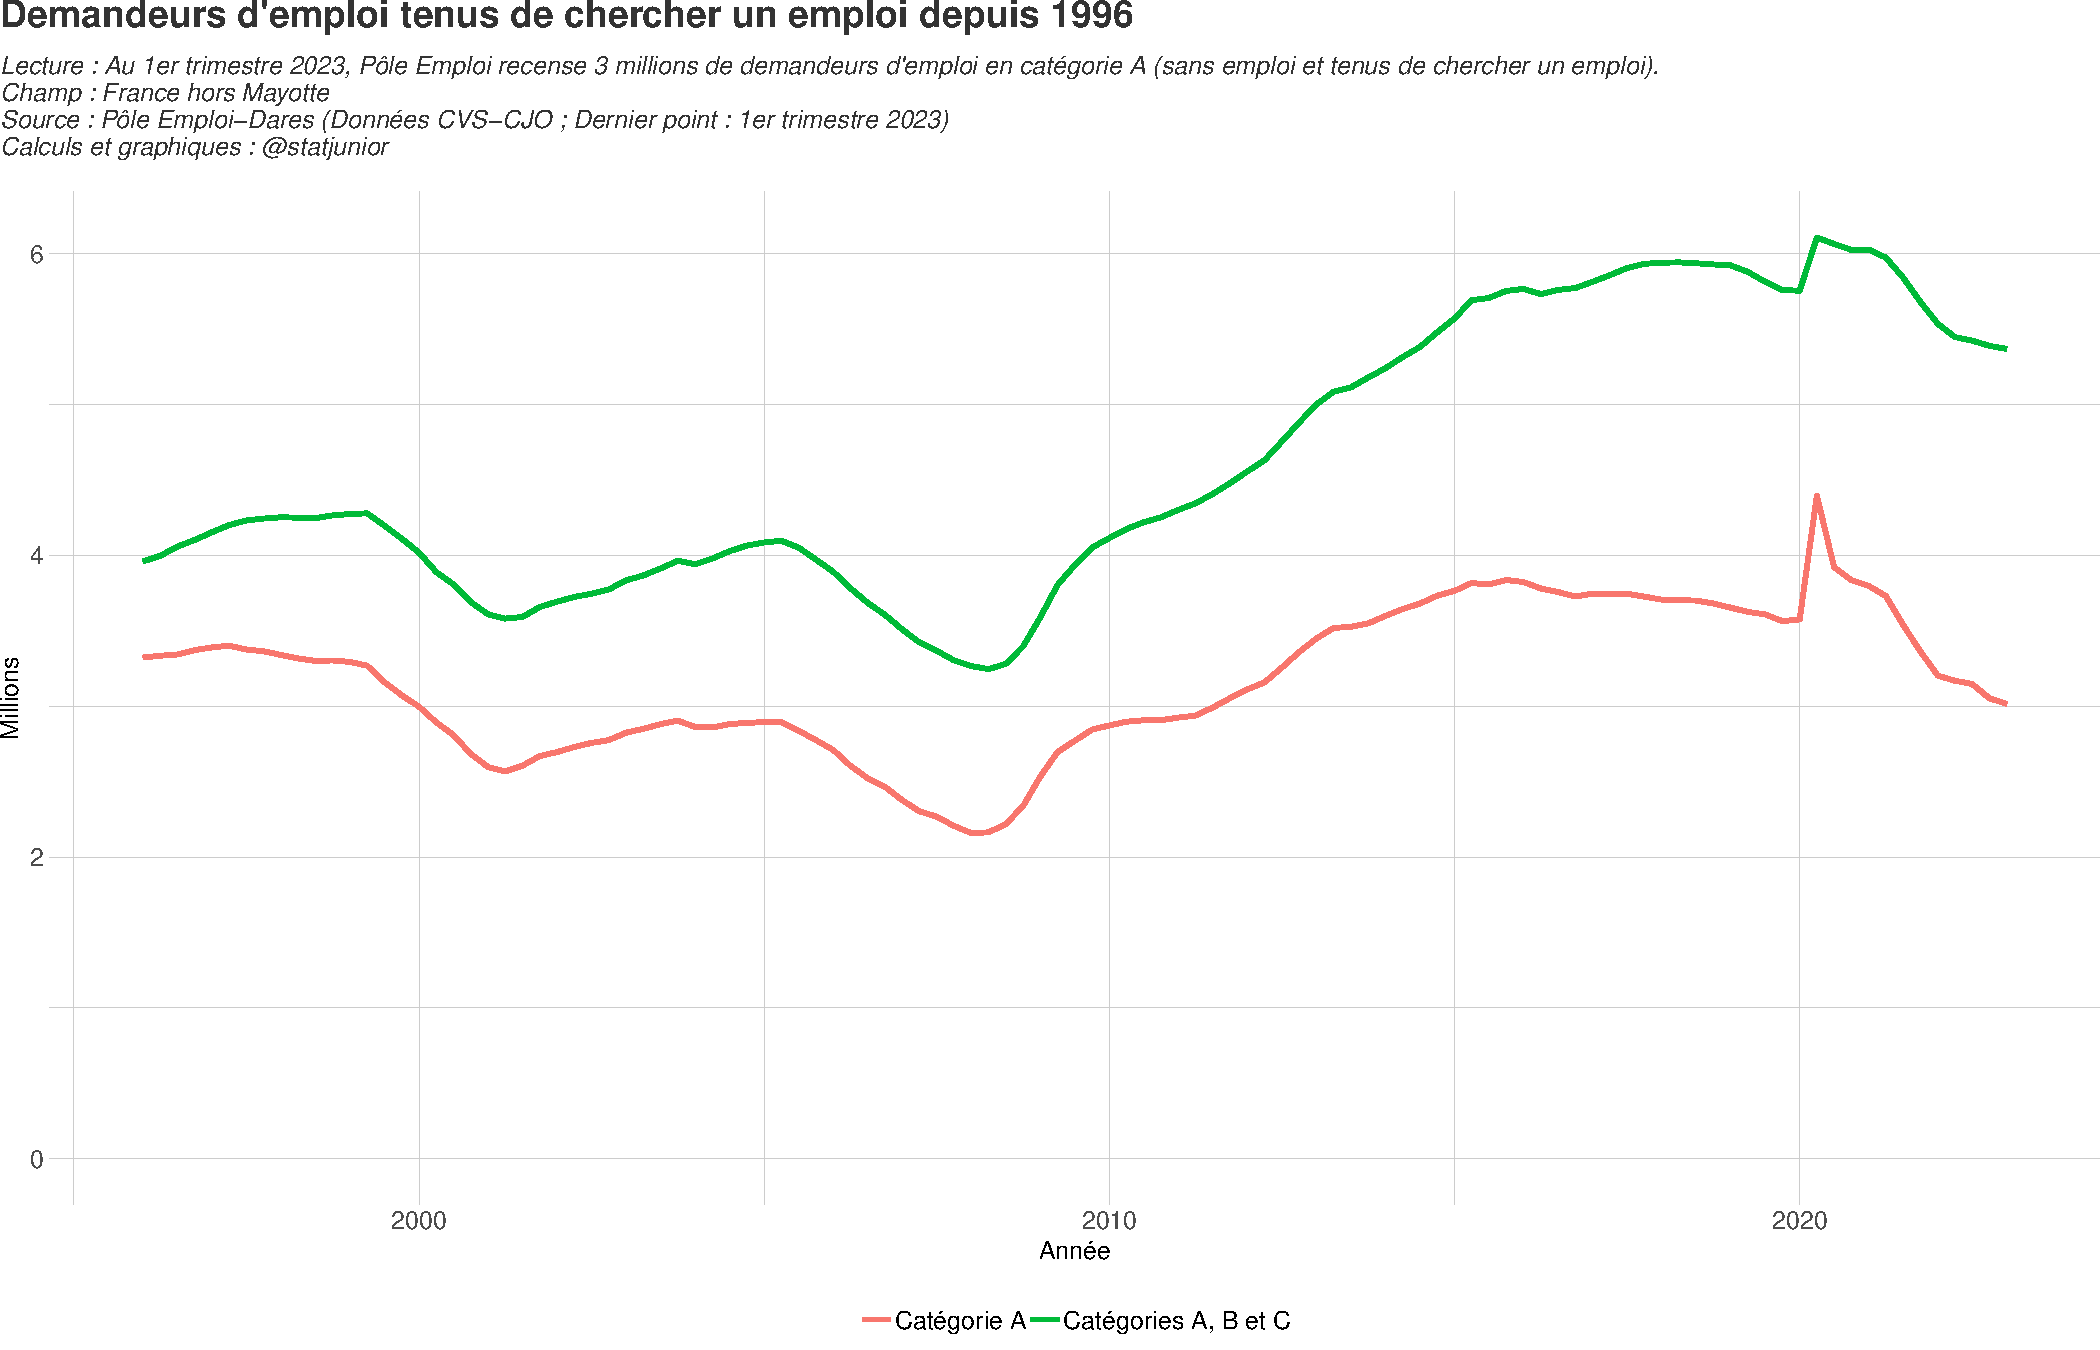
\includegraphics[keepaspectratio]{rapport_pdf_demandeurs_emploi_pole_emploi_files/figure-latex/unnamed-chunk-2-1.pdf}}

\subsection{Catégorie A, A-B-C et toutes catégories en France
métropolitaine}\label{catuxe9gorie-a-a-b-c-et-toutes-catuxe9gories-en-france-muxe9tropolitaine}

\pandocbounded{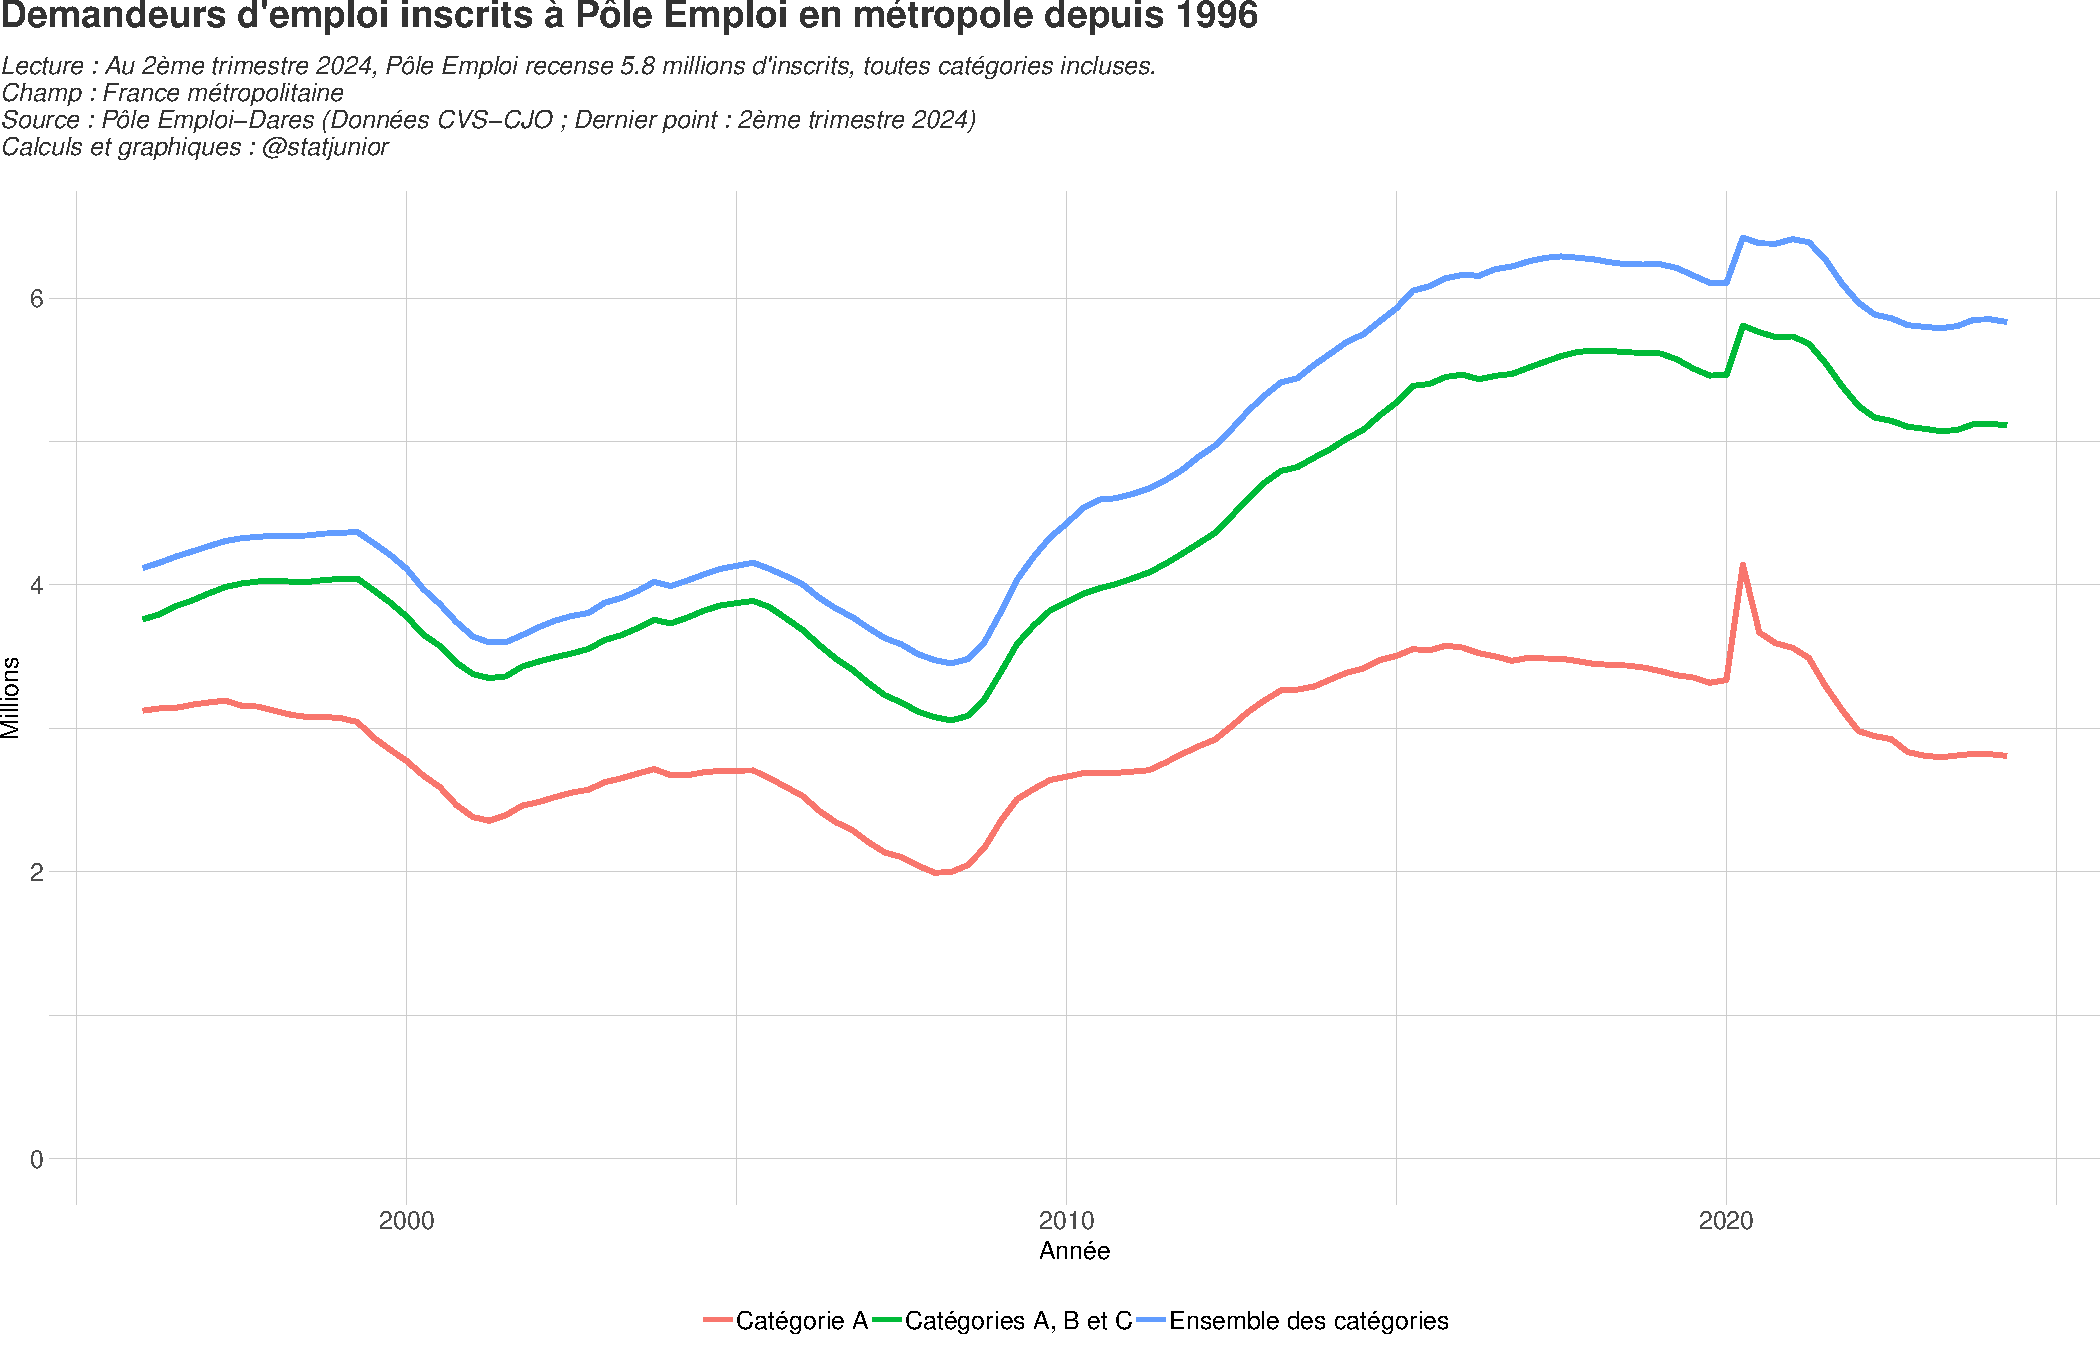
\includegraphics[keepaspectratio]{rapport_pdf_demandeurs_emploi_pole_emploi_files/figure-latex/unnamed-chunk-3-1.pdf}}

\newpage

\subsection{Variation trimestrielle et annuelle des demandeurs
d'emploi}\label{variation-trimestrielle-et-annuelle-des-demandeurs-demploi}

Au 2ème trimestre 2024, le nombre de demandeurs d'emploi en catégorie A
baisse de -0.4 \% par rapport au trimestre précédent et augmente de
0.2\% sur un an.

Le nombre de demandeurs d'emploi en catégories A-B-C baisse de -0.2 \%
par rapport au trimestre précédent et augmente de 0.8\% sur un an.

Le nombre de demandeurs d'emploi toutes catégories comprises baisse de
-0.3 \% par rapport au trimestre précédent et augmente de 0.7\% sur un
an.

\pandocbounded{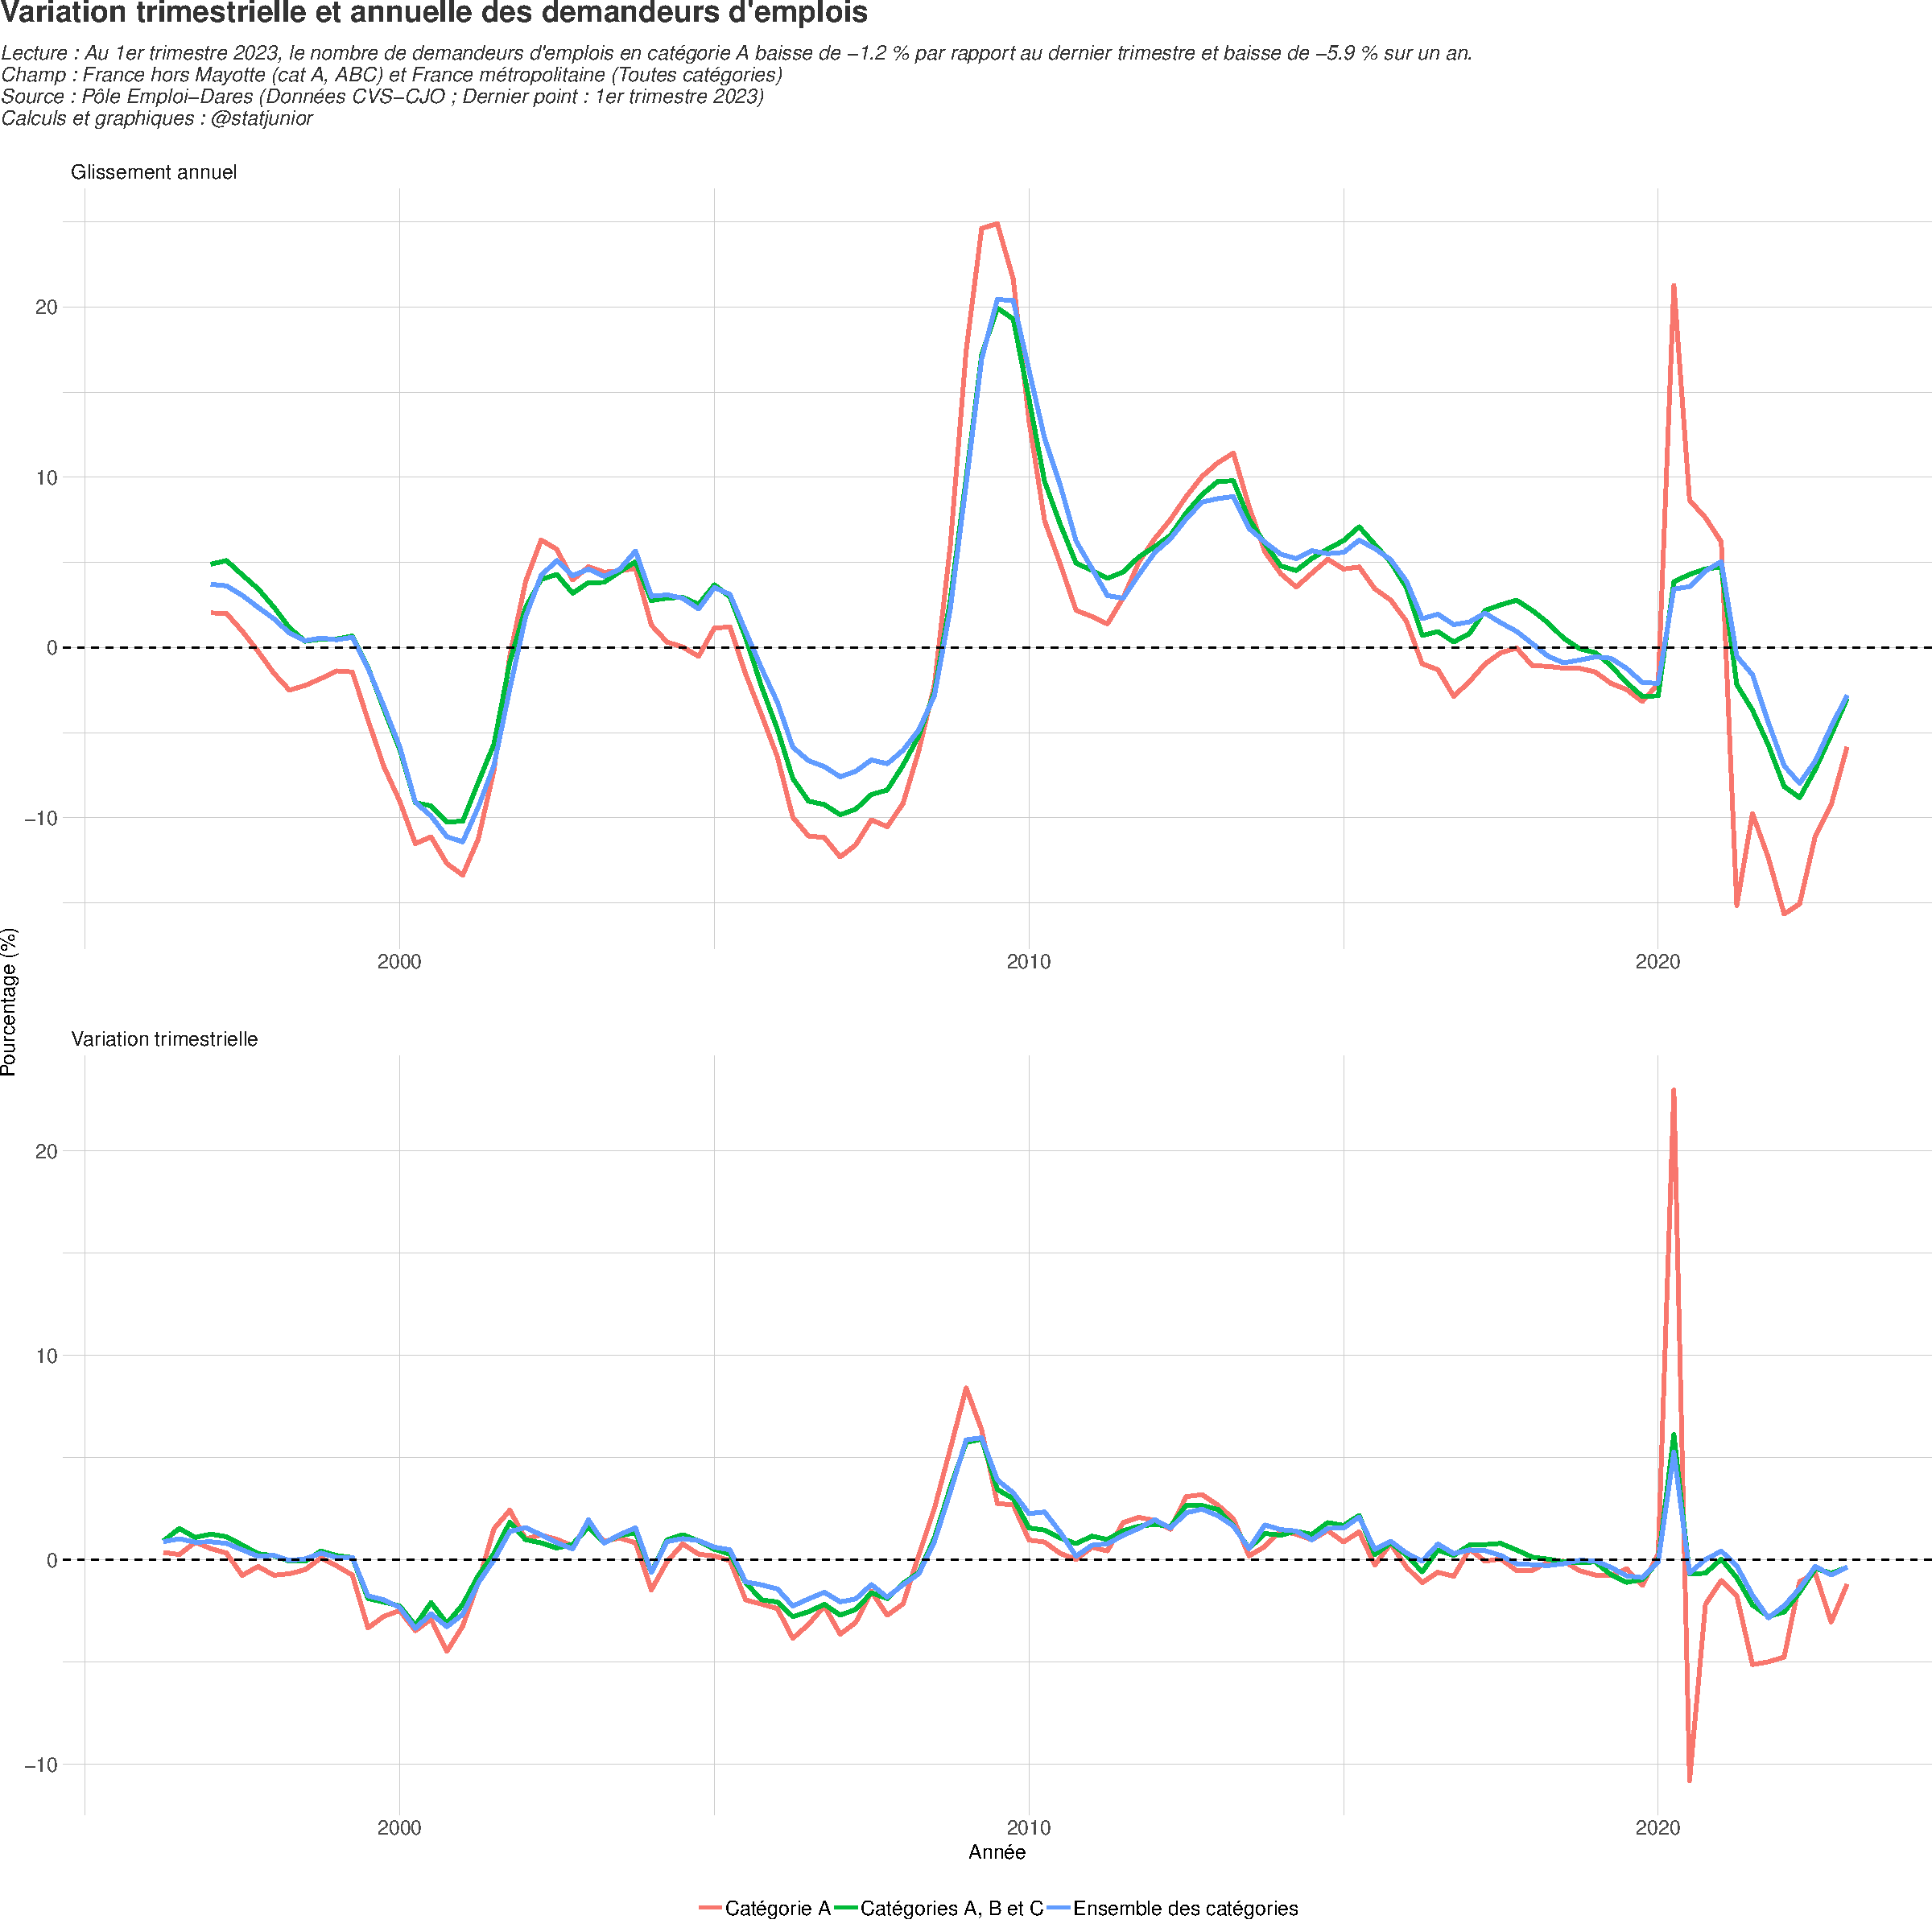
\includegraphics[keepaspectratio]{rapport_pdf_demandeurs_emploi_pole_emploi_files/figure-latex/unnamed-chunk-5-1.pdf}}

\section{Structure des inscrits par genre et par tranche
d'âge}\label{structure-des-inscrits-par-genre-et-par-tranche-duxe2ge}

\subsection{Par genre (catégorie A et catégorie
A-B-C)}\label{par-genre-catuxe9gorie-a-et-catuxe9gorie-a-b-c}

\pandocbounded{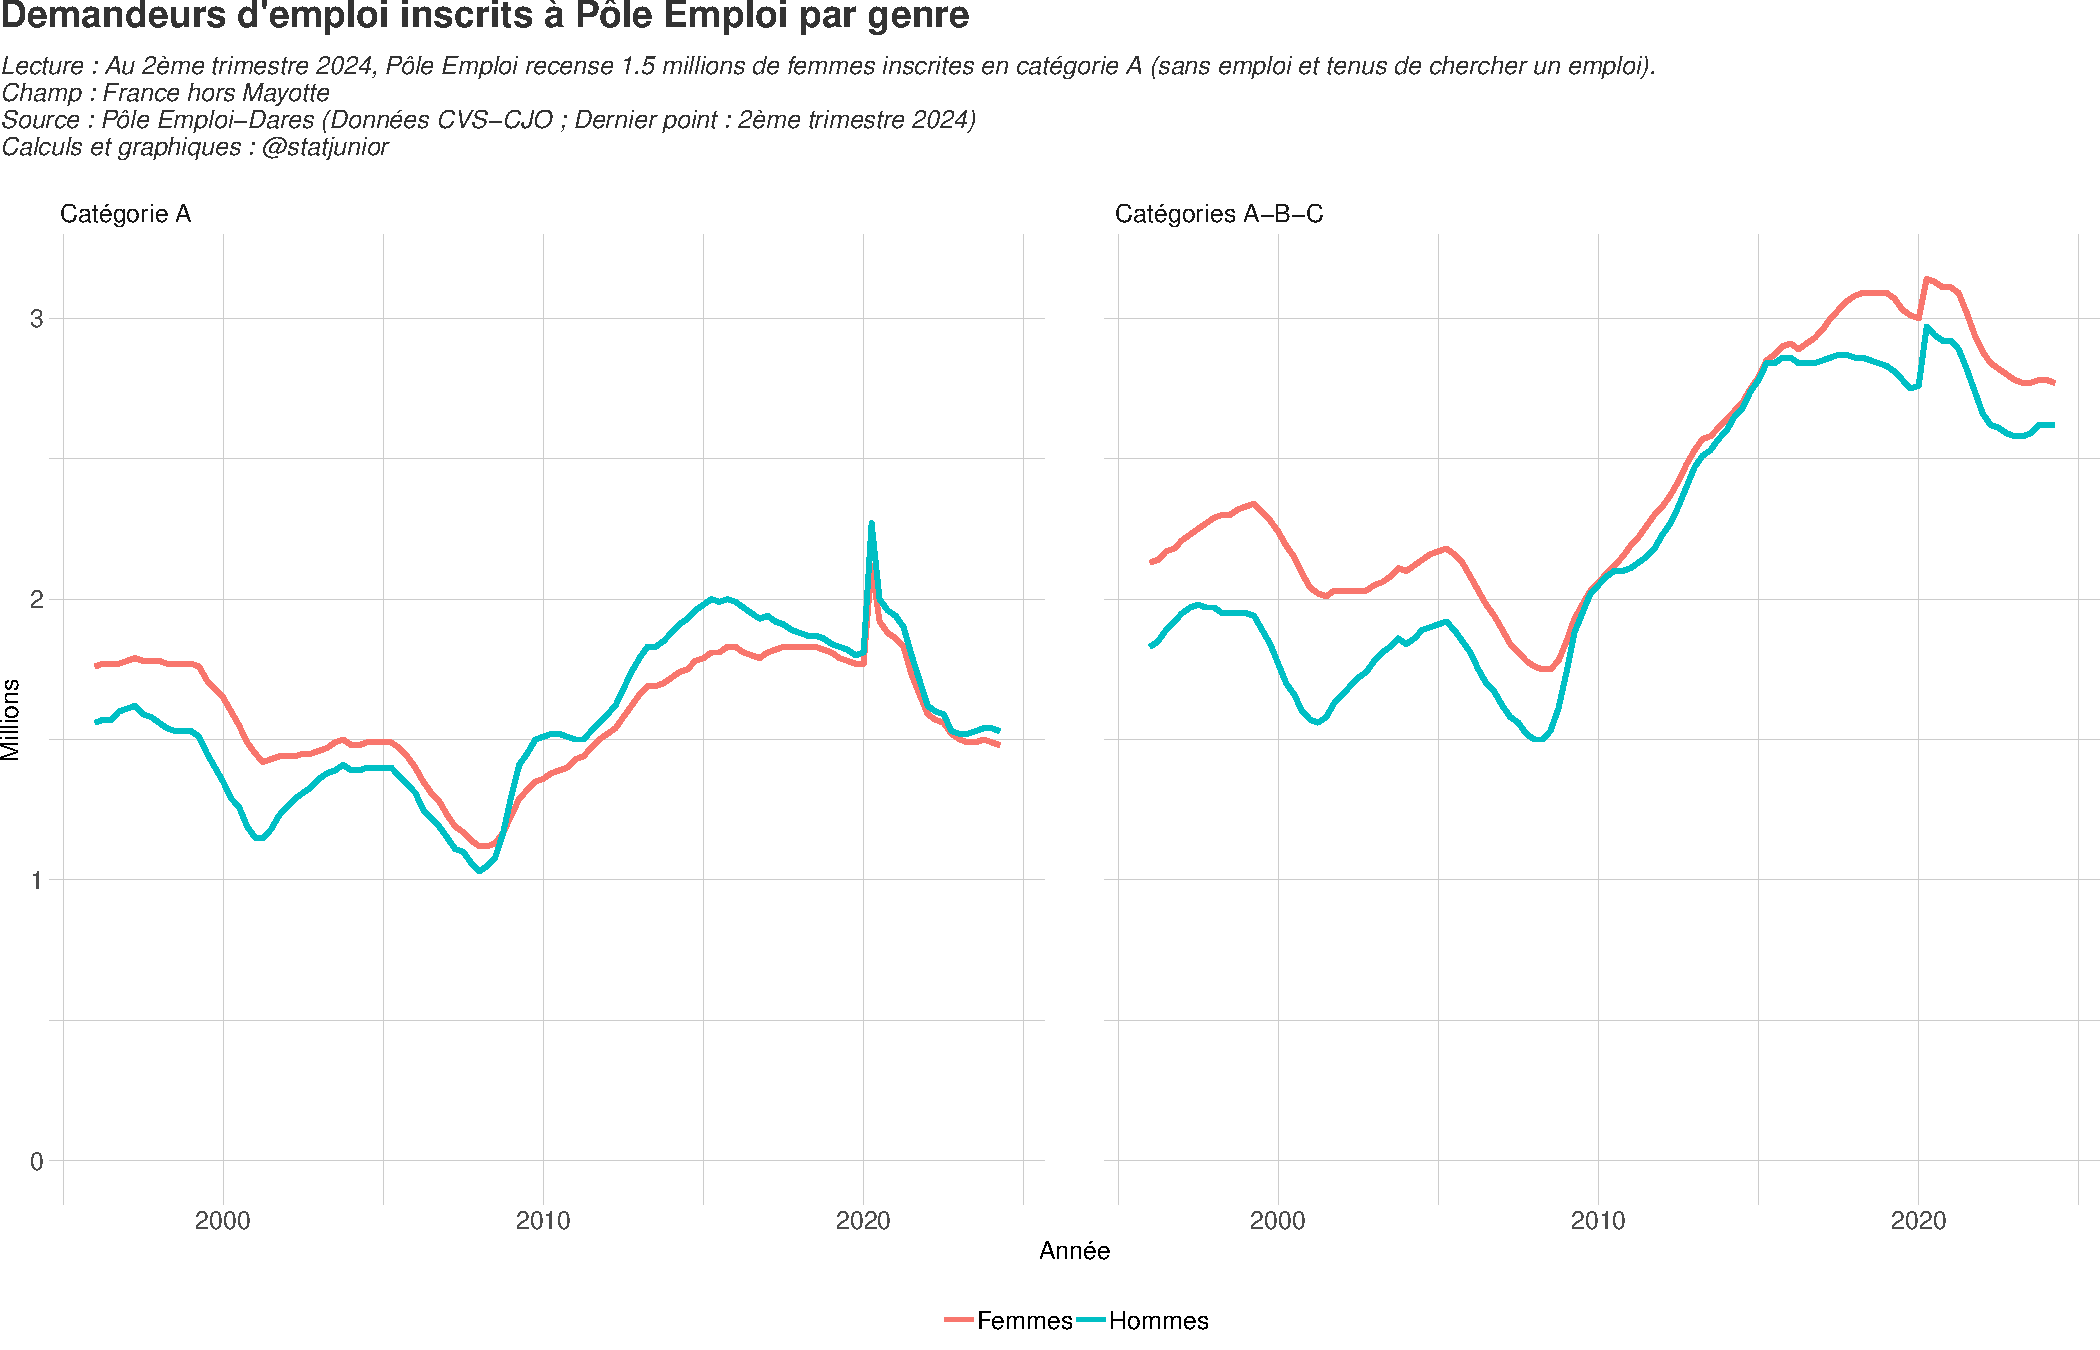
\includegraphics[keepaspectratio]{rapport_pdf_demandeurs_emploi_pole_emploi_files/figure-latex/unnamed-chunk-7-1.pdf}}

\subsection{Par tranche d'âge (catégorie A et catégorie
A-B-C)}\label{par-tranche-duxe2ge-catuxe9gorie-a-et-catuxe9gorie-a-b-c}

\pandocbounded{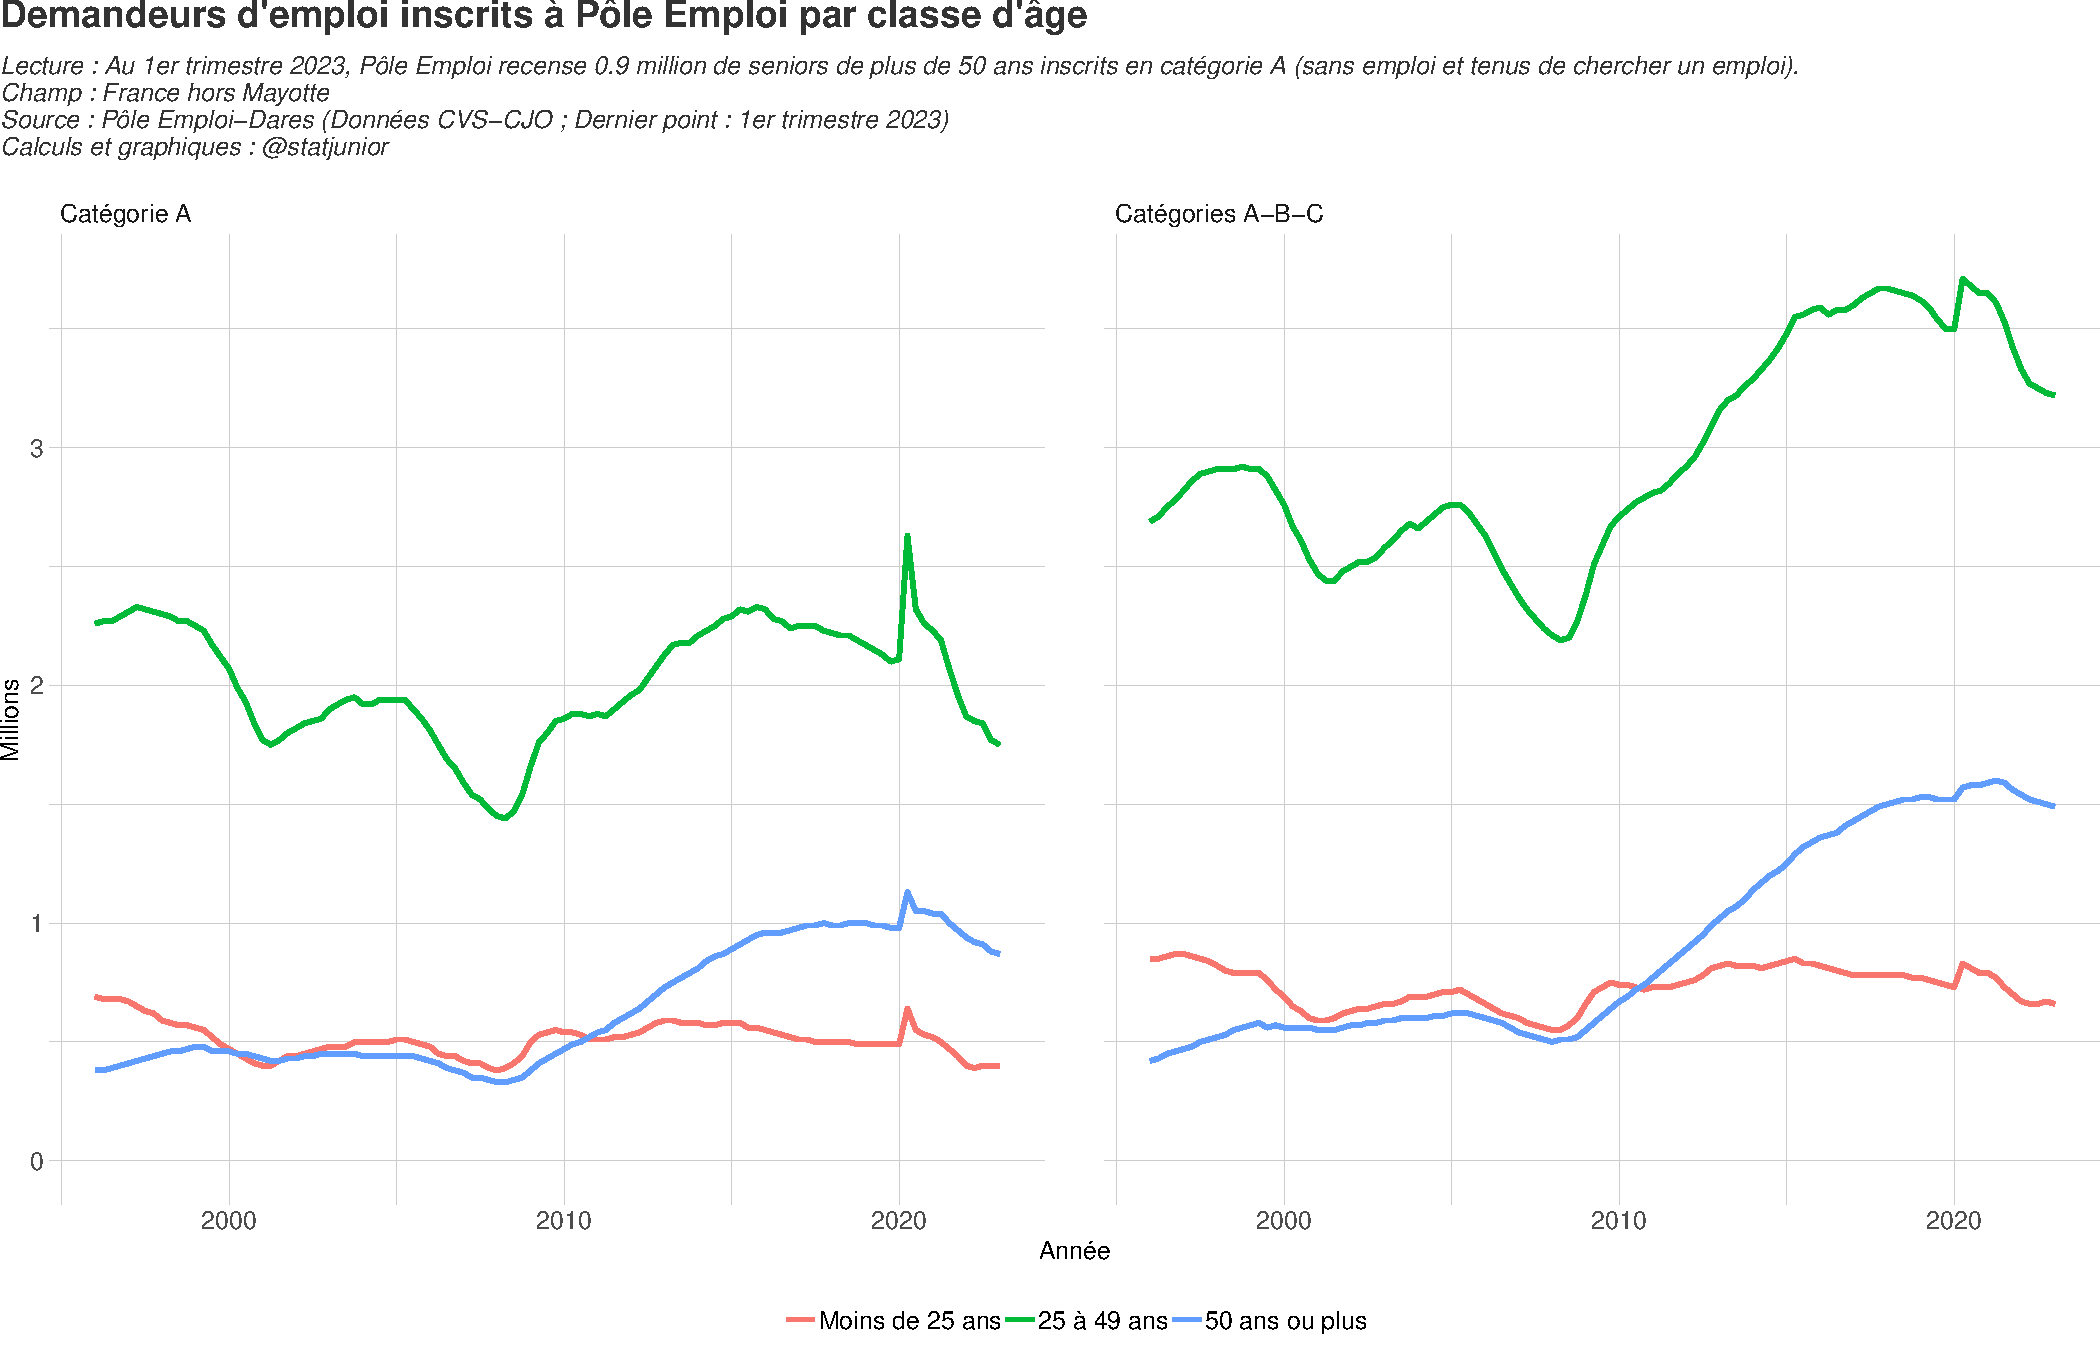
\includegraphics[keepaspectratio]{rapport_pdf_demandeurs_emploi_pole_emploi_files/figure-latex/unnamed-chunk-9-1.pdf}}

\section{Ancienneté d'inscription à Pôle
Emploi}\label{anciennetuxe9-dinscription-uxe0-puxf4le-emploi}

\subsection{Parmi les inscrits au 2ème trimestre
2024}\label{parmi-les-inscrits-au-2uxe8me-trimestre-2024}

\pandocbounded{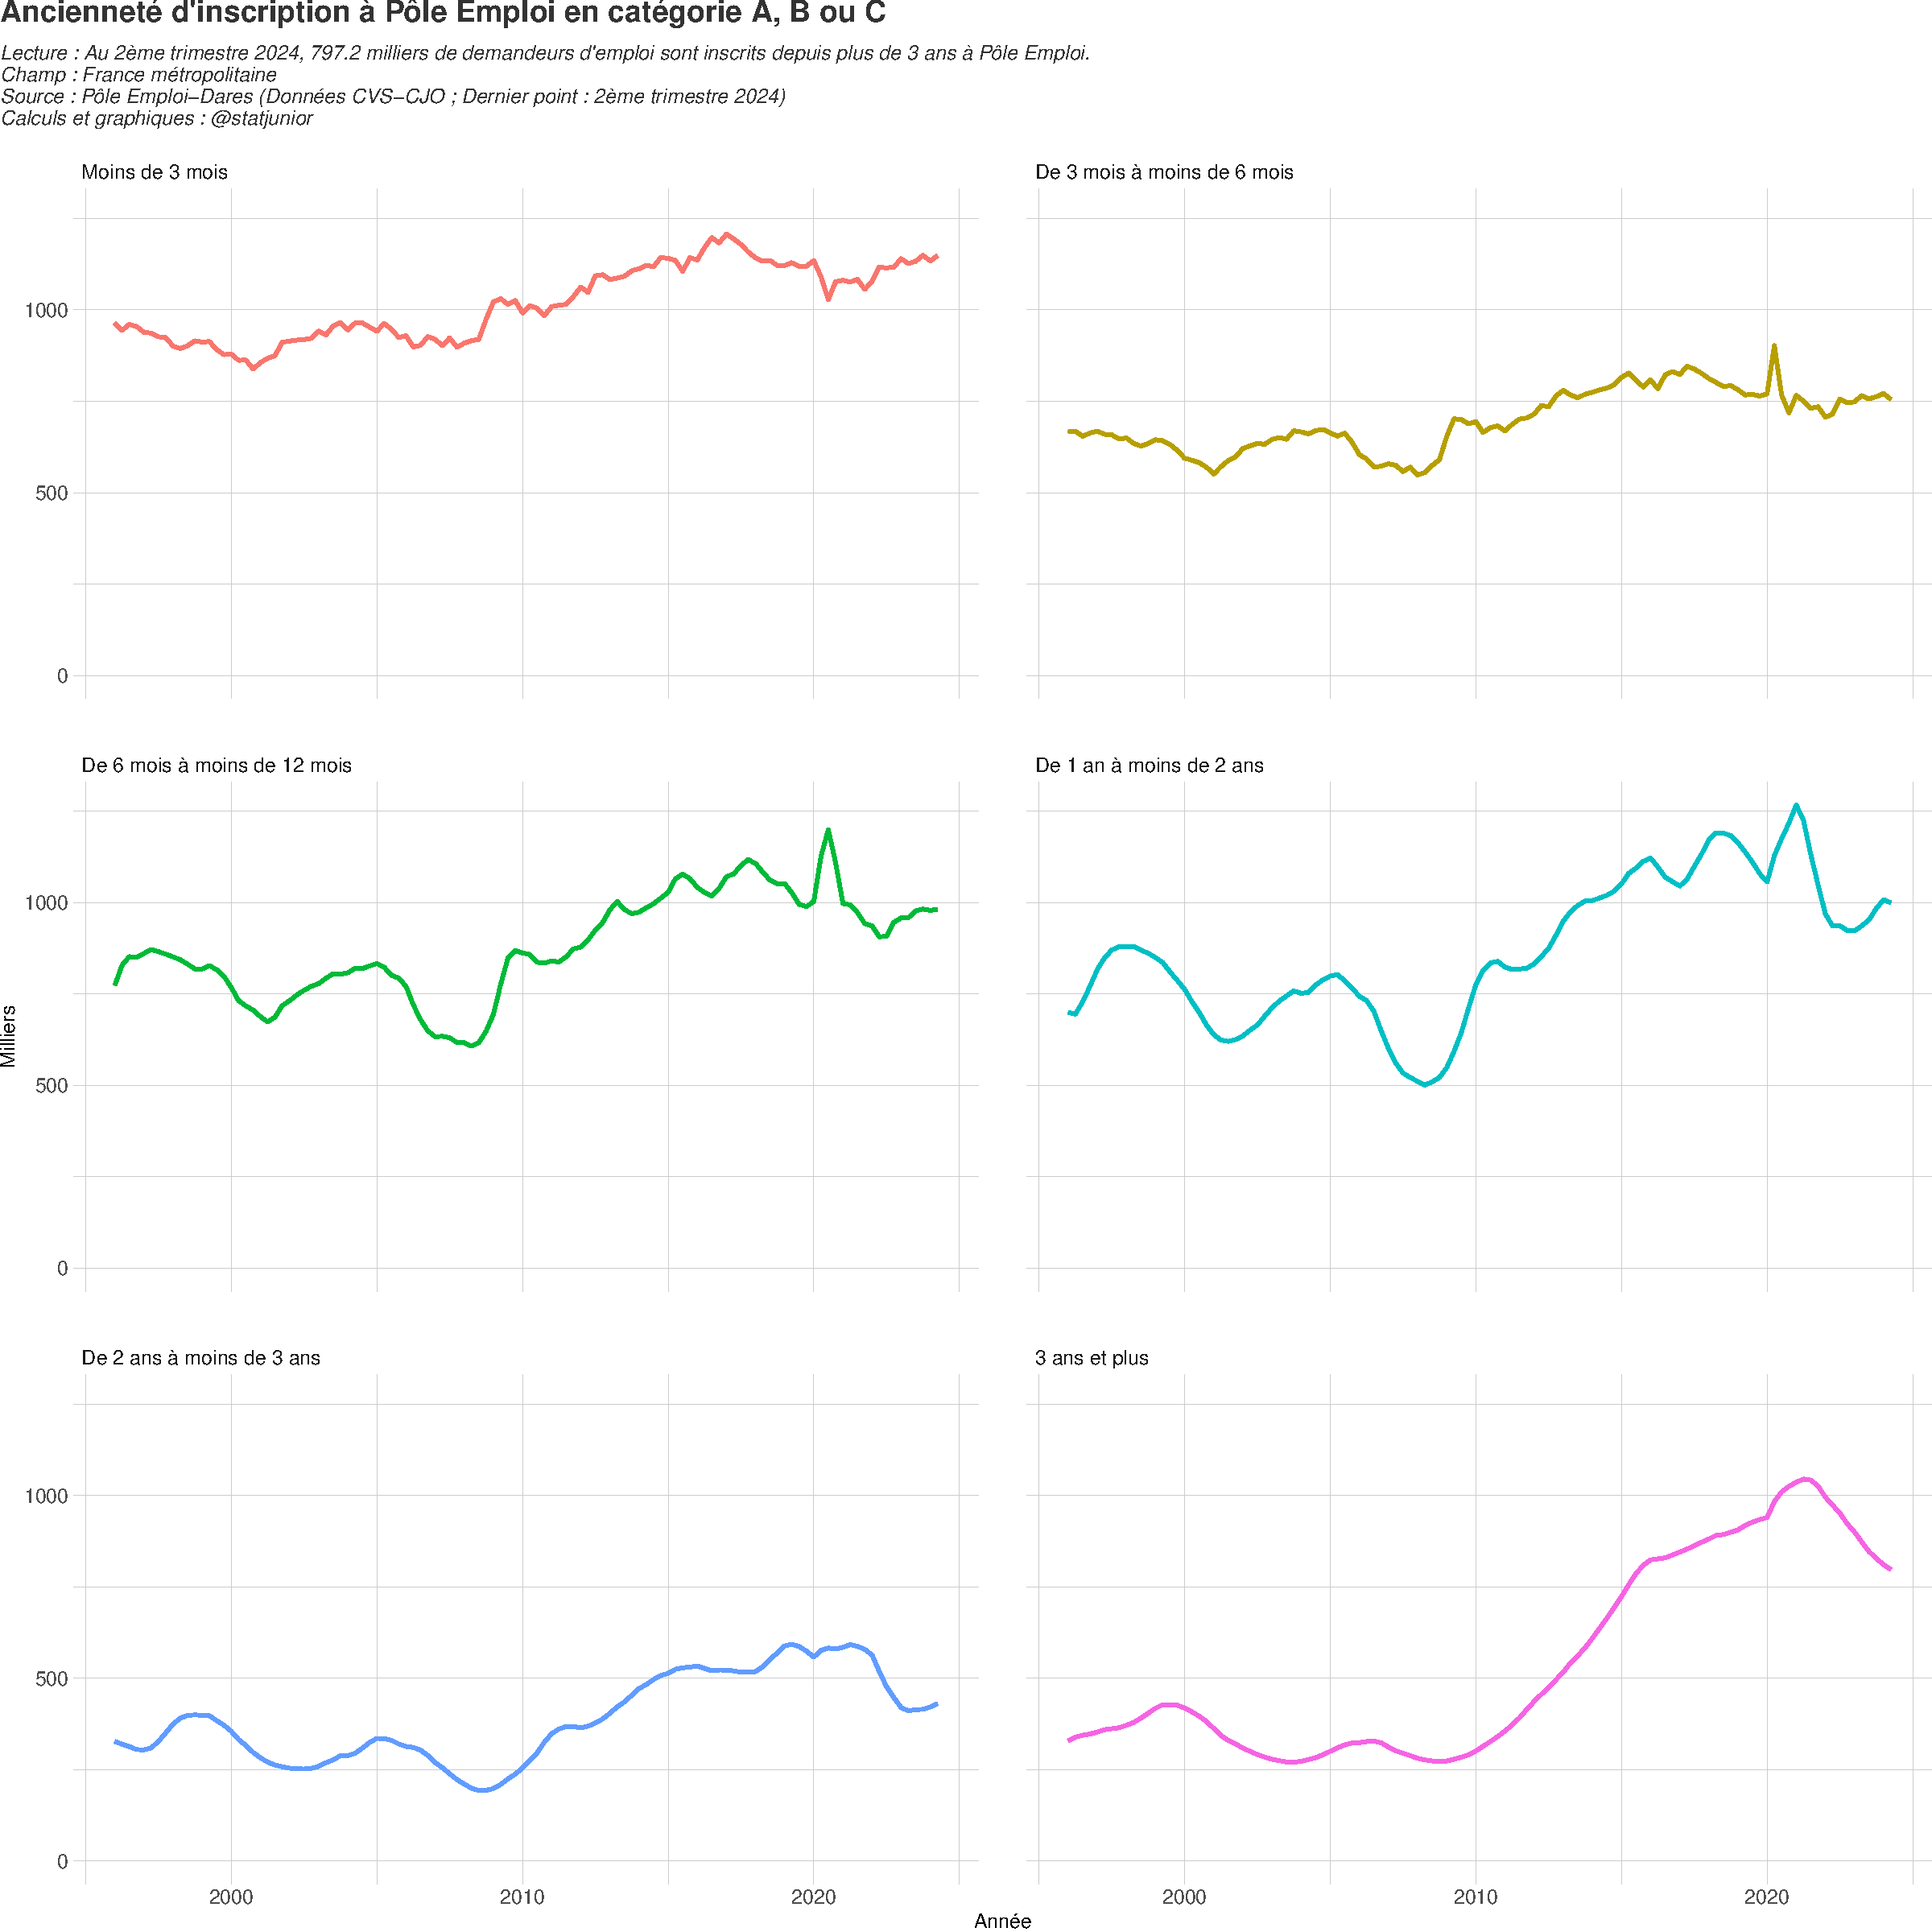
\includegraphics[keepaspectratio]{rapport_pdf_demandeurs_emploi_pole_emploi_files/figure-latex/unnamed-chunk-11-1.pdf}}

\subsection{Par tranche d'âge (en distinguant les inscrits des sortants
au 2ème trimestre
2024)}\label{par-tranche-duxe2ge-en-distinguant-les-inscrits-des-sortants-au-2uxe8me-trimestre-2024}

\pandocbounded{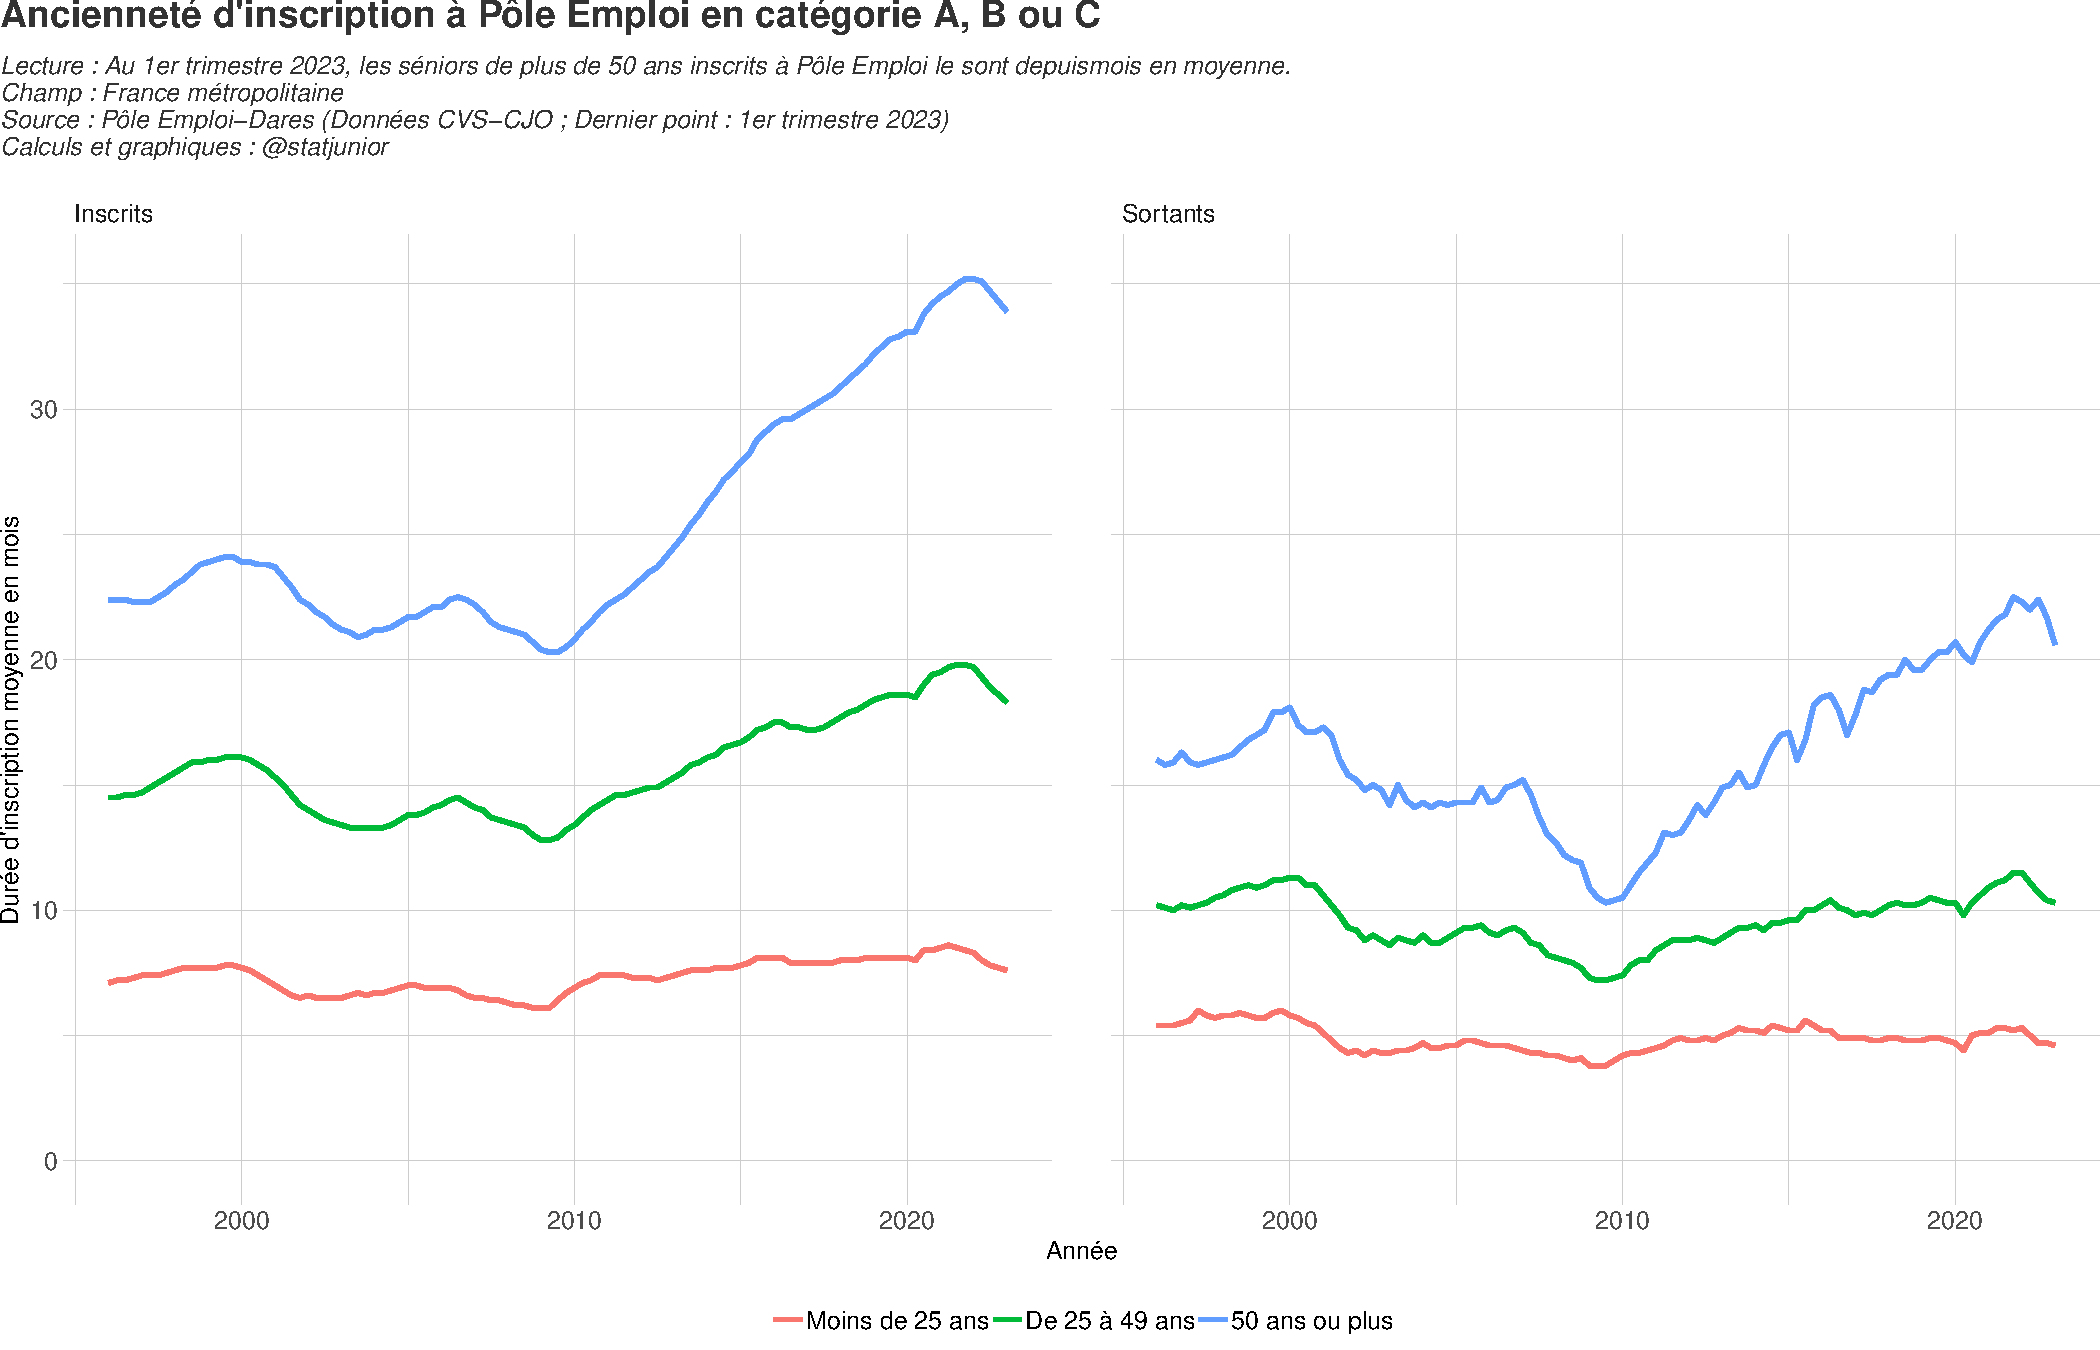
\includegraphics[keepaspectratio]{rapport_pdf_demandeurs_emploi_pole_emploi_files/figure-latex/unnamed-chunk-13-1.pdf}}

\section{Les motifs d'entrée à Pôle Emploi au 2ème trimestre
2024}\label{les-motifs-dentruxe9e-uxe0-puxf4le-emploi-au-2uxe8me-trimestre-2024}

\pandocbounded{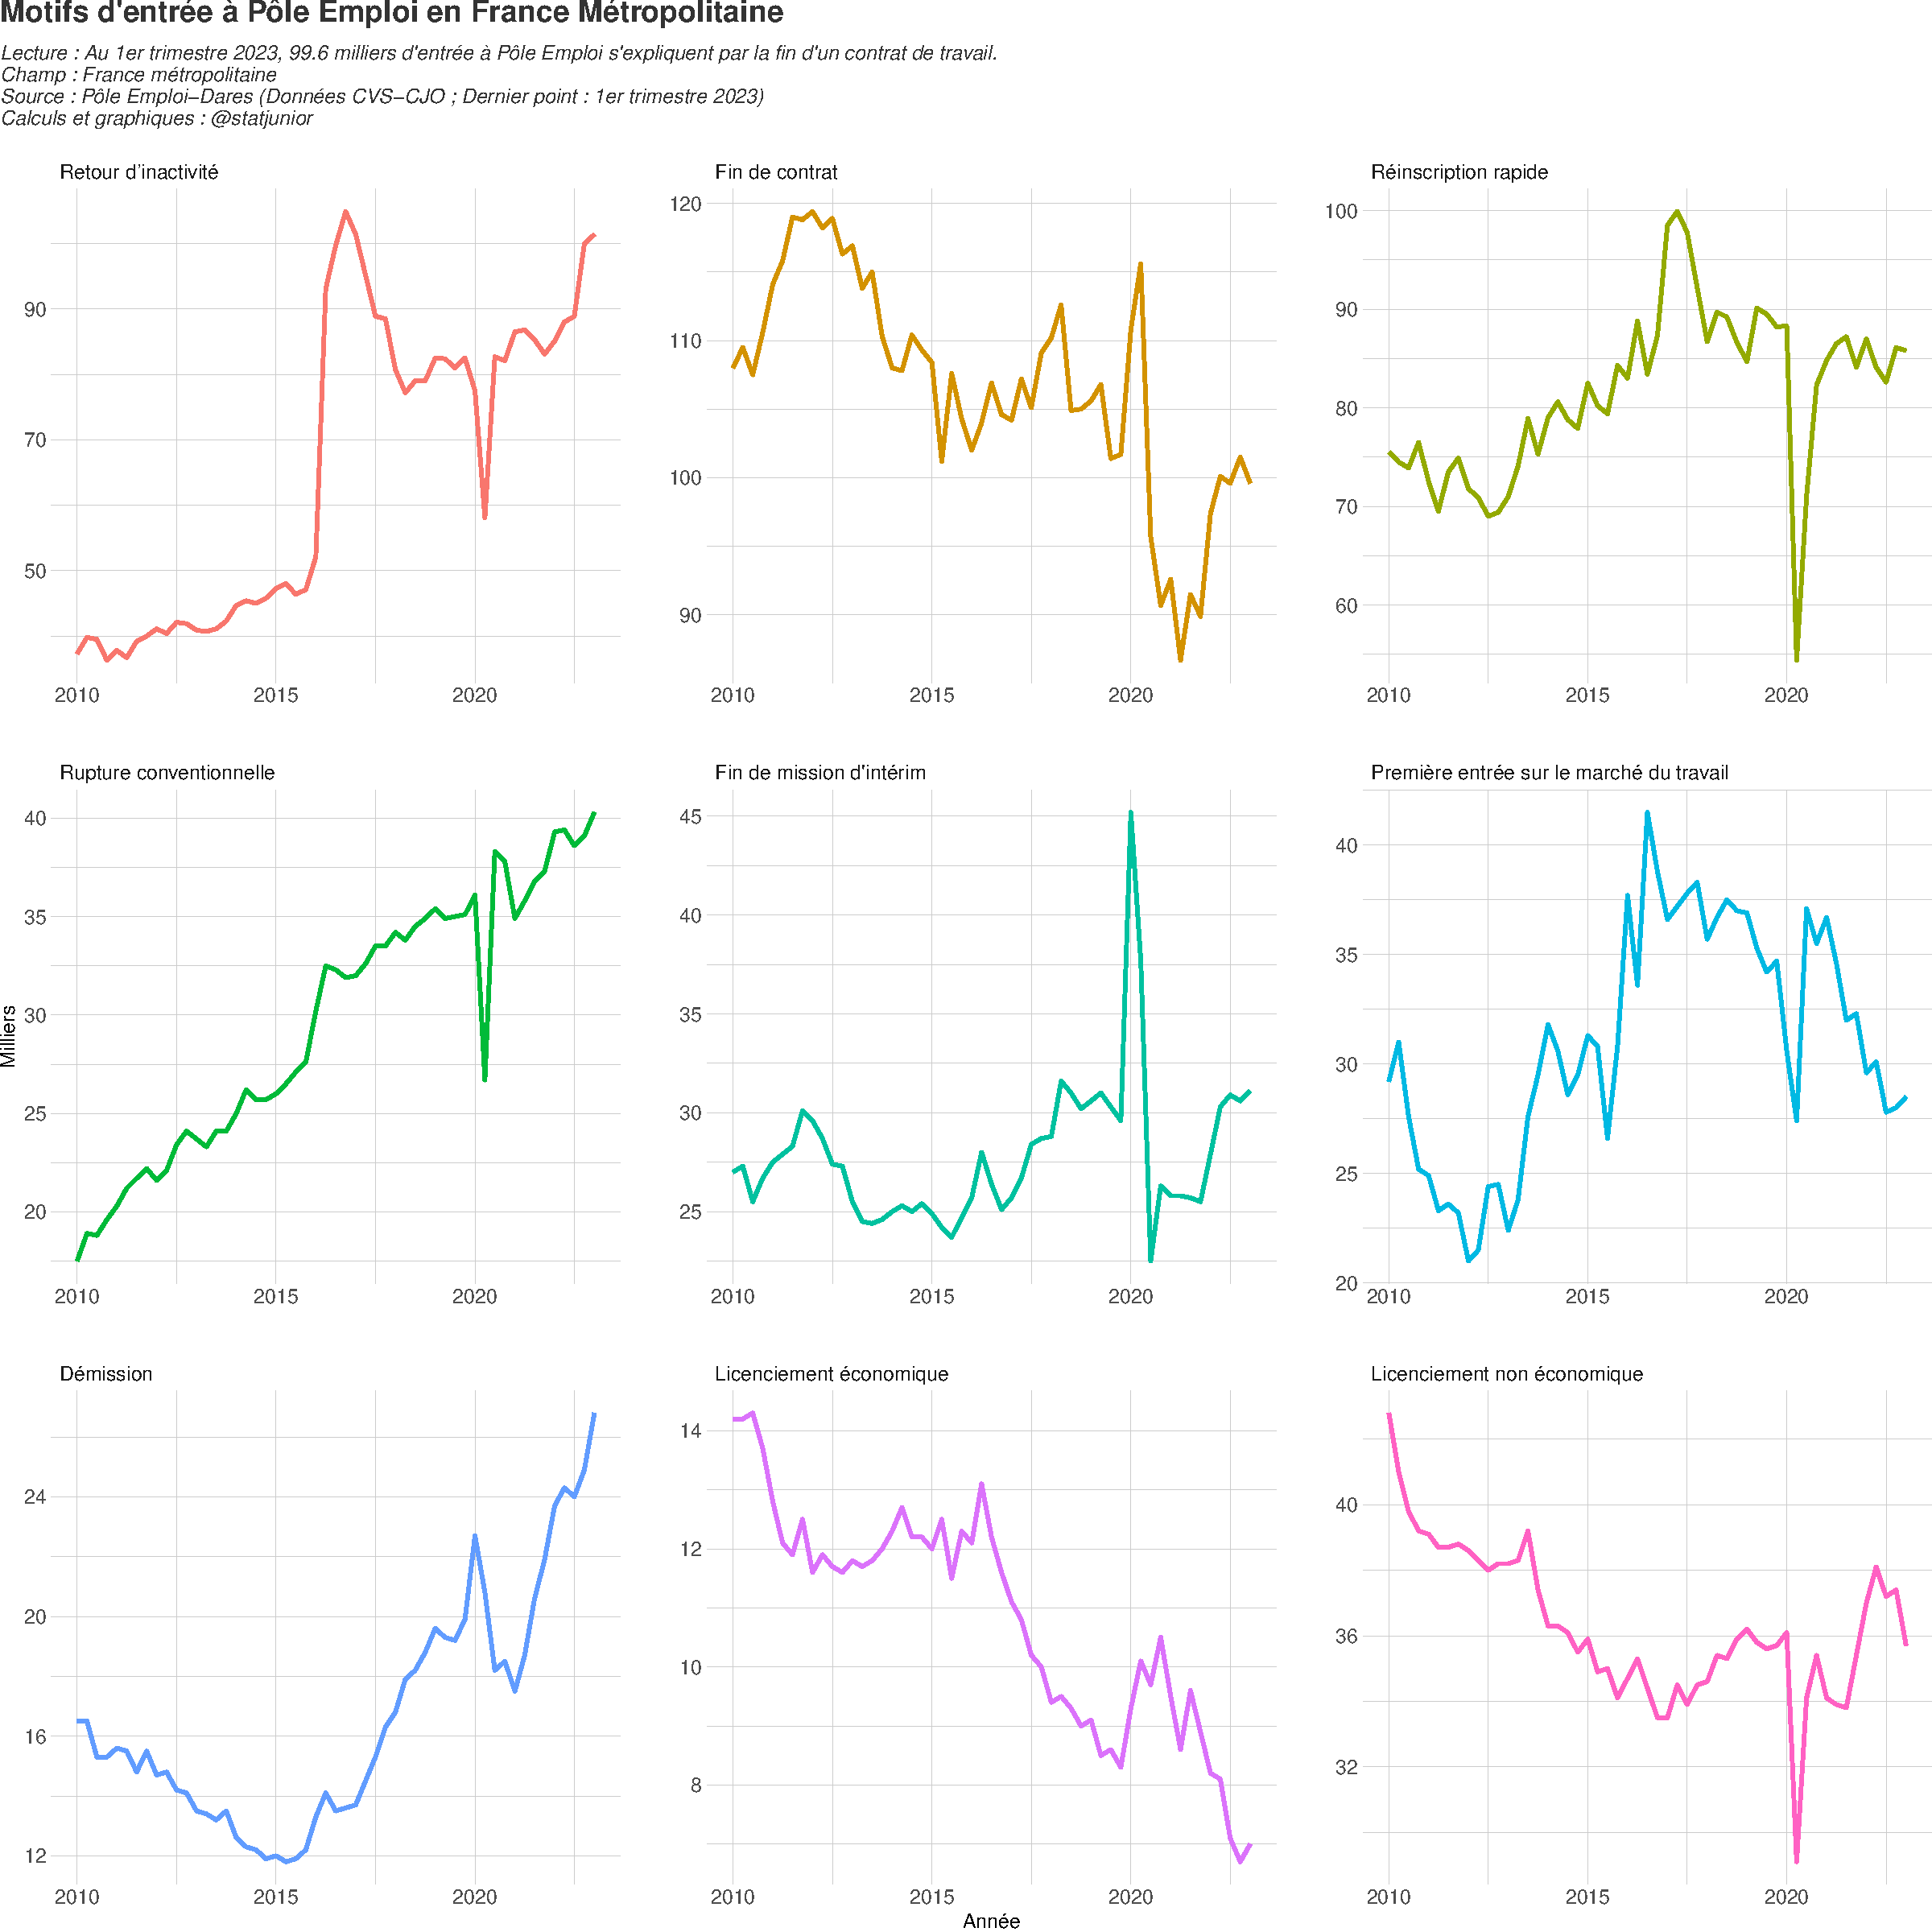
\includegraphics[keepaspectratio]{rapport_pdf_demandeurs_emploi_pole_emploi_files/figure-latex/unnamed-chunk-15-1.pdf}}

\section{Les motifs de sortie de Pôle Emploi au 2ème trimestre
2024}\label{les-motifs-de-sortie-de-puxf4le-emploi-au-2uxe8me-trimestre-2024}

\pandocbounded{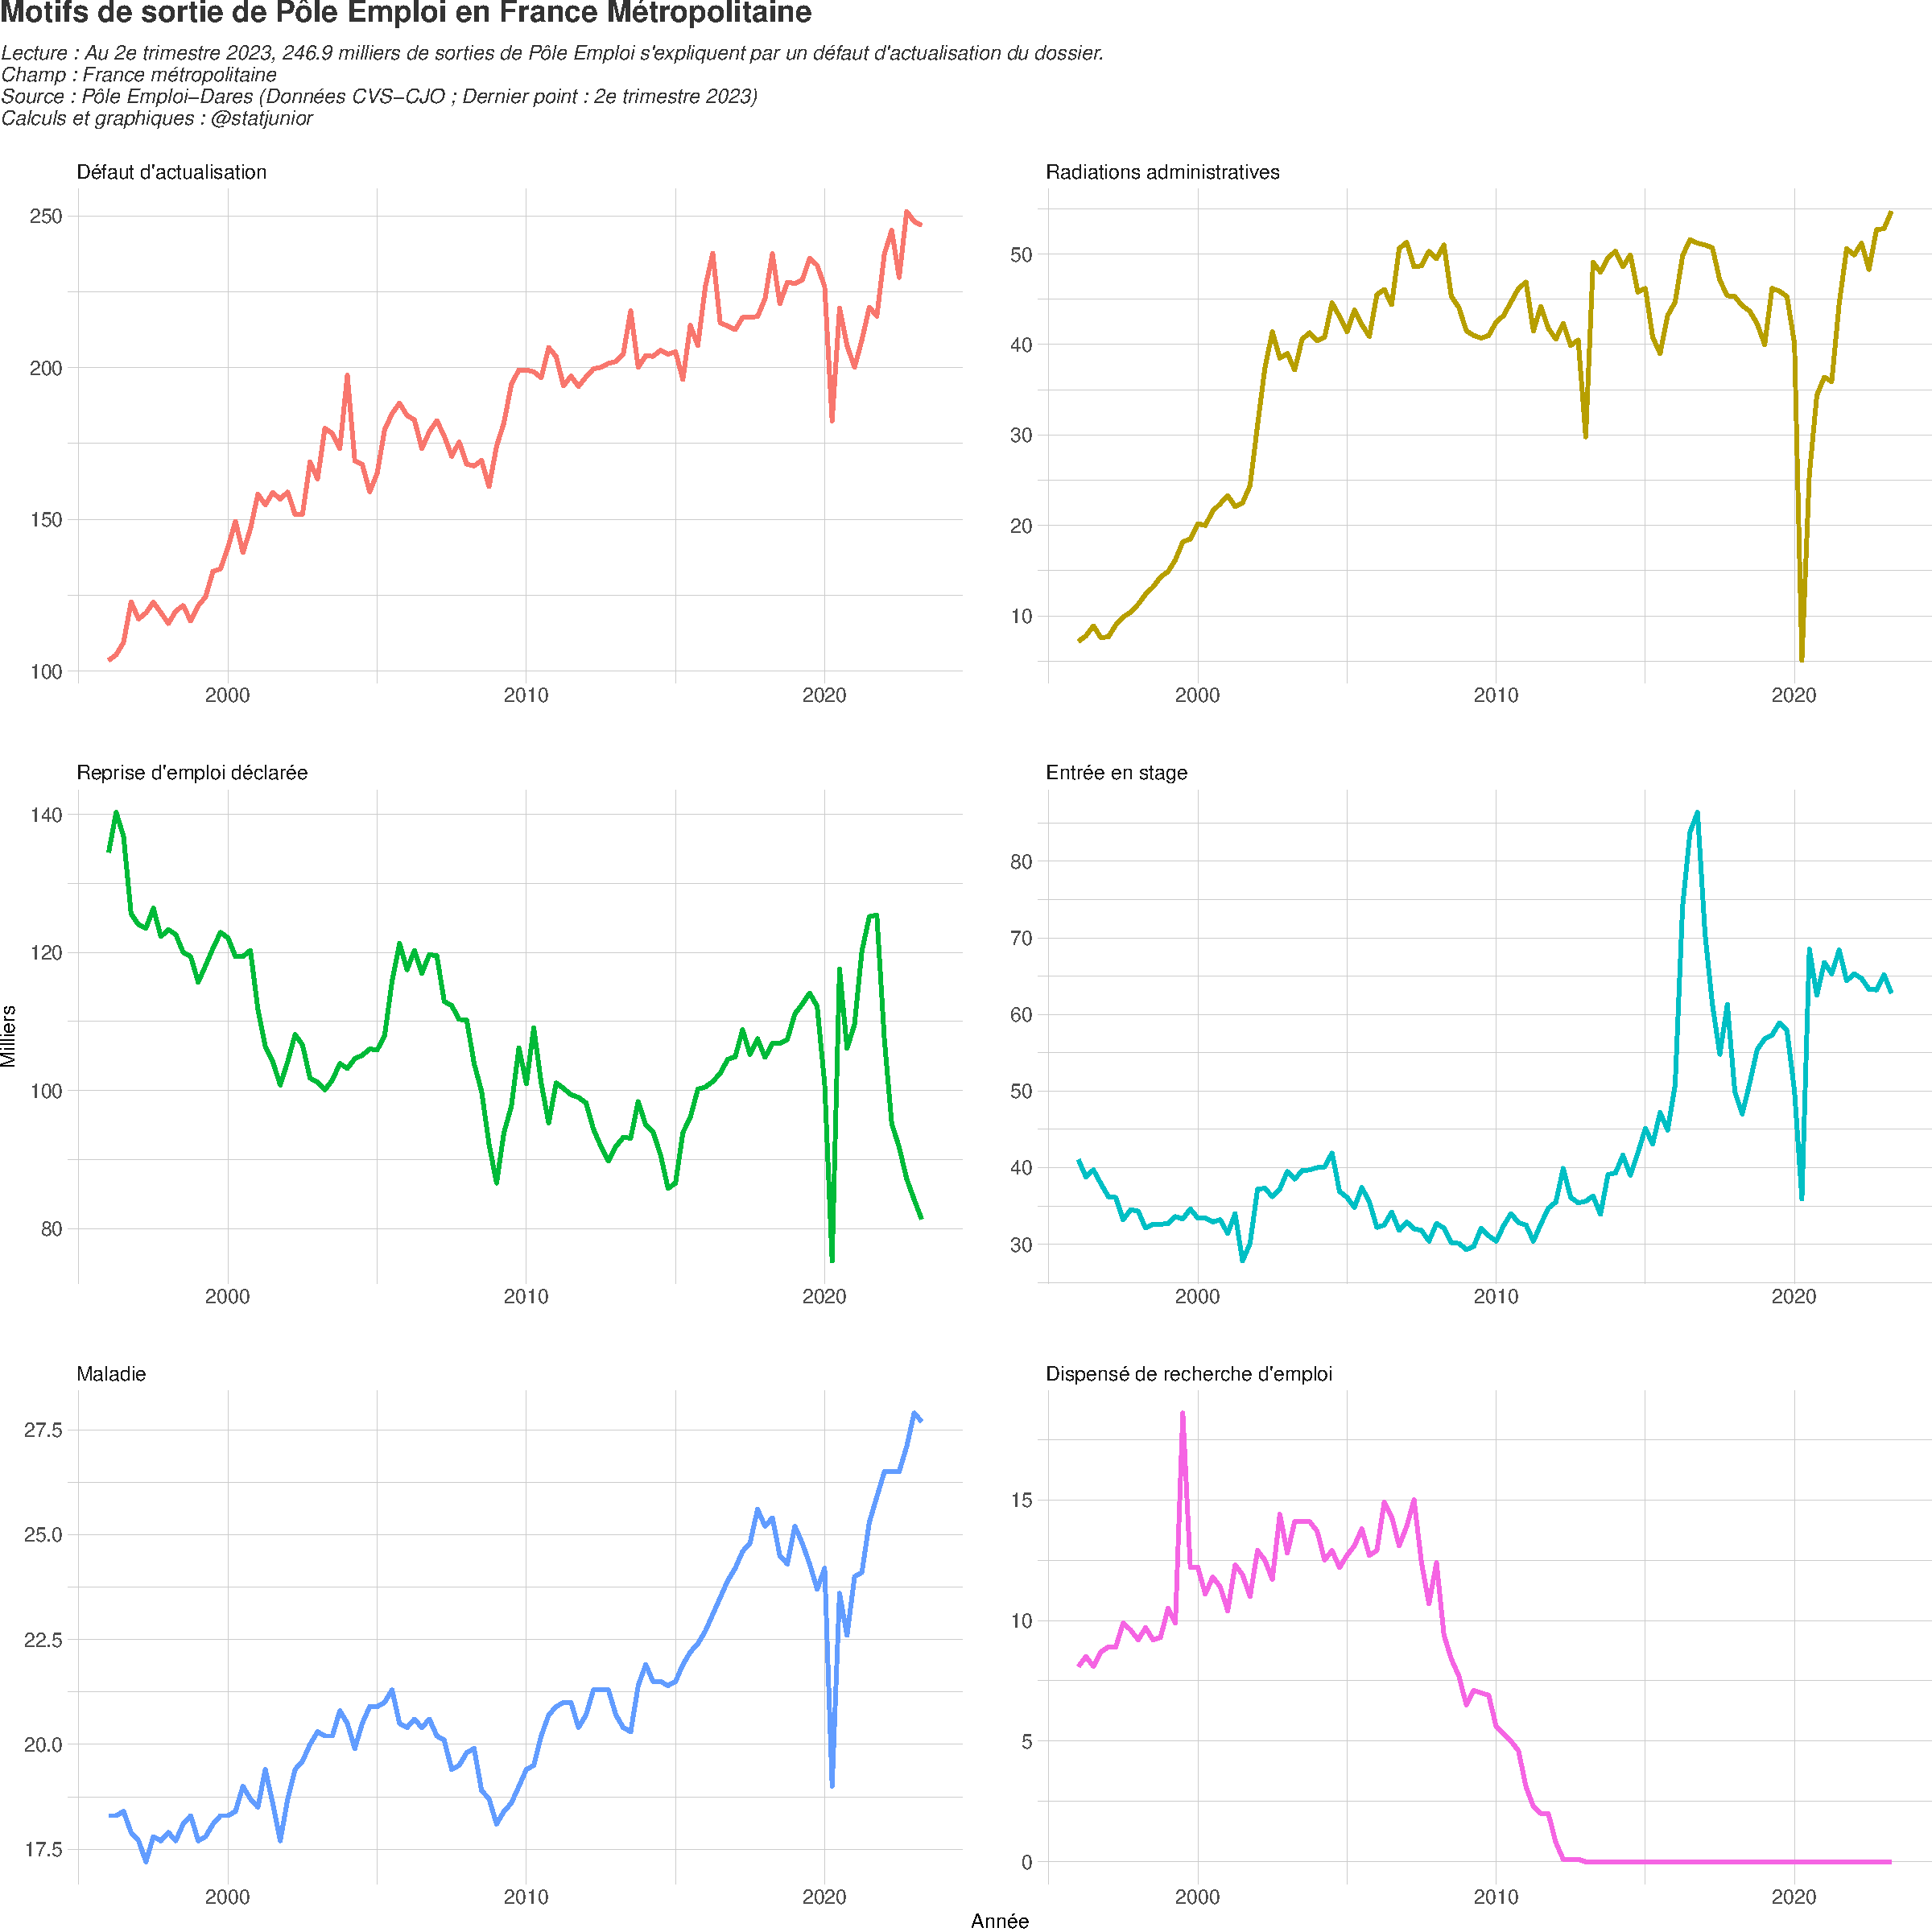
\includegraphics[keepaspectratio]{rapport_pdf_demandeurs_emploi_pole_emploi_files/figure-latex/unnamed-chunk-17-1.pdf}}

\newpage

\section{Les allocataires indemnisés par Pôle
Emploi}\label{les-allocataires-indemnisuxe9s-par-puxf4le-emploi}

Attention : dernier point au 3e trimestre 2023.

\pandocbounded{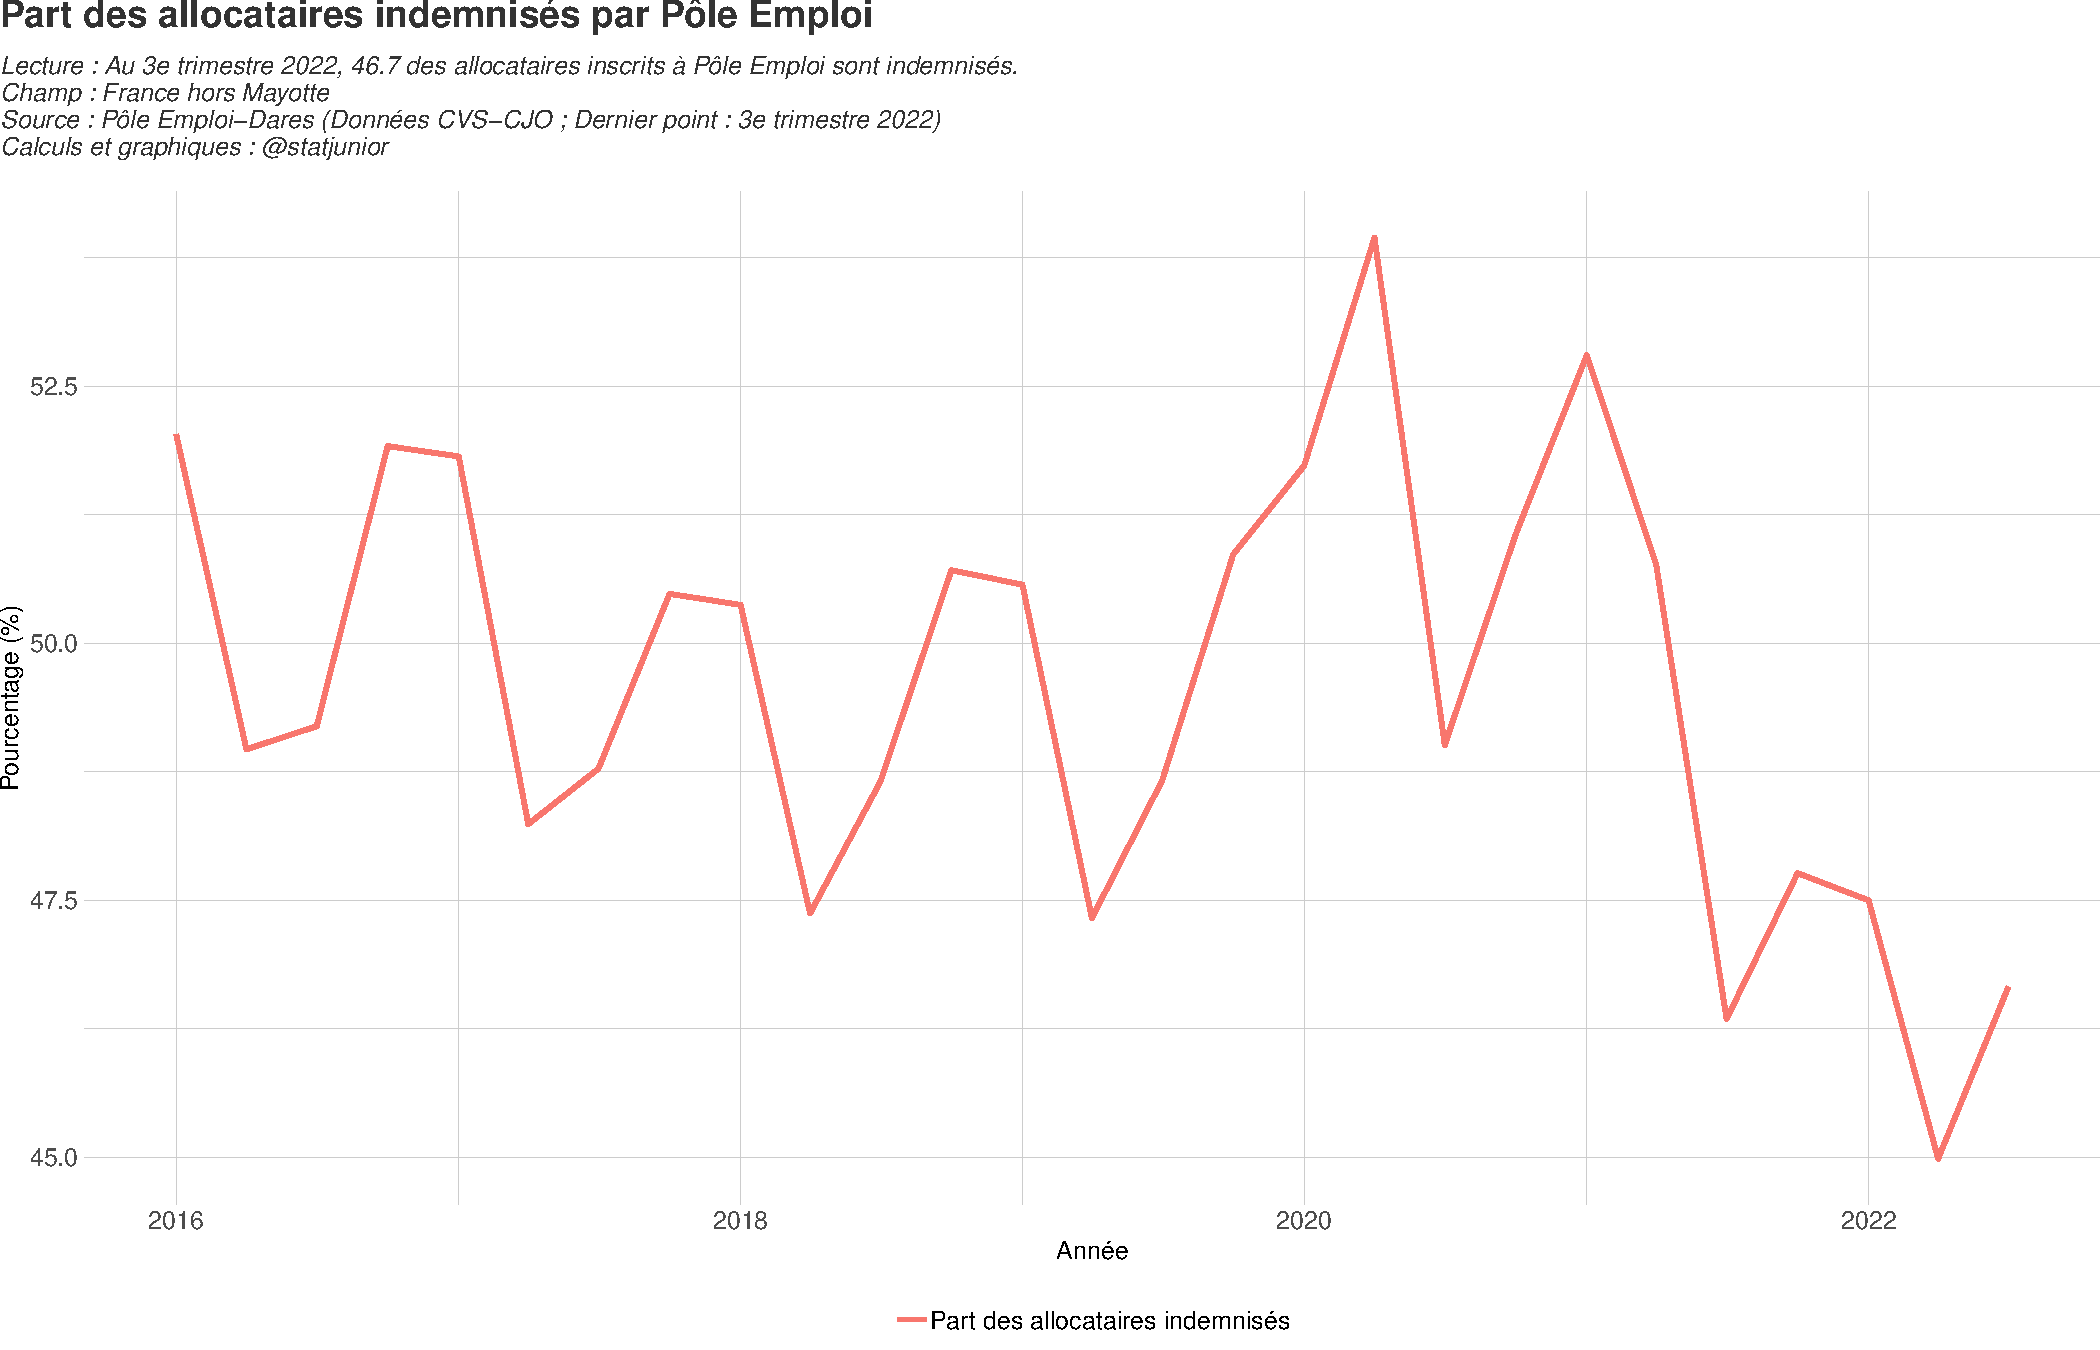
\includegraphics[keepaspectratio]{rapport_pdf_demandeurs_emploi_pole_emploi_files/figure-latex/unnamed-chunk-19-1.pdf}}

\newpage

\section{La confrontation des sources administratives (Dares-Pôle
Emploi) avec l'enquête Emploi (chômage
BIT-Insee)}\label{la-confrontation-des-sources-administratives-dares-puxf4le-emploi-avec-lenquuxeate-emploi-chuxf4mage-bit-insee}

Attention : dernier point au 1er trimestre 2024.

\pandocbounded{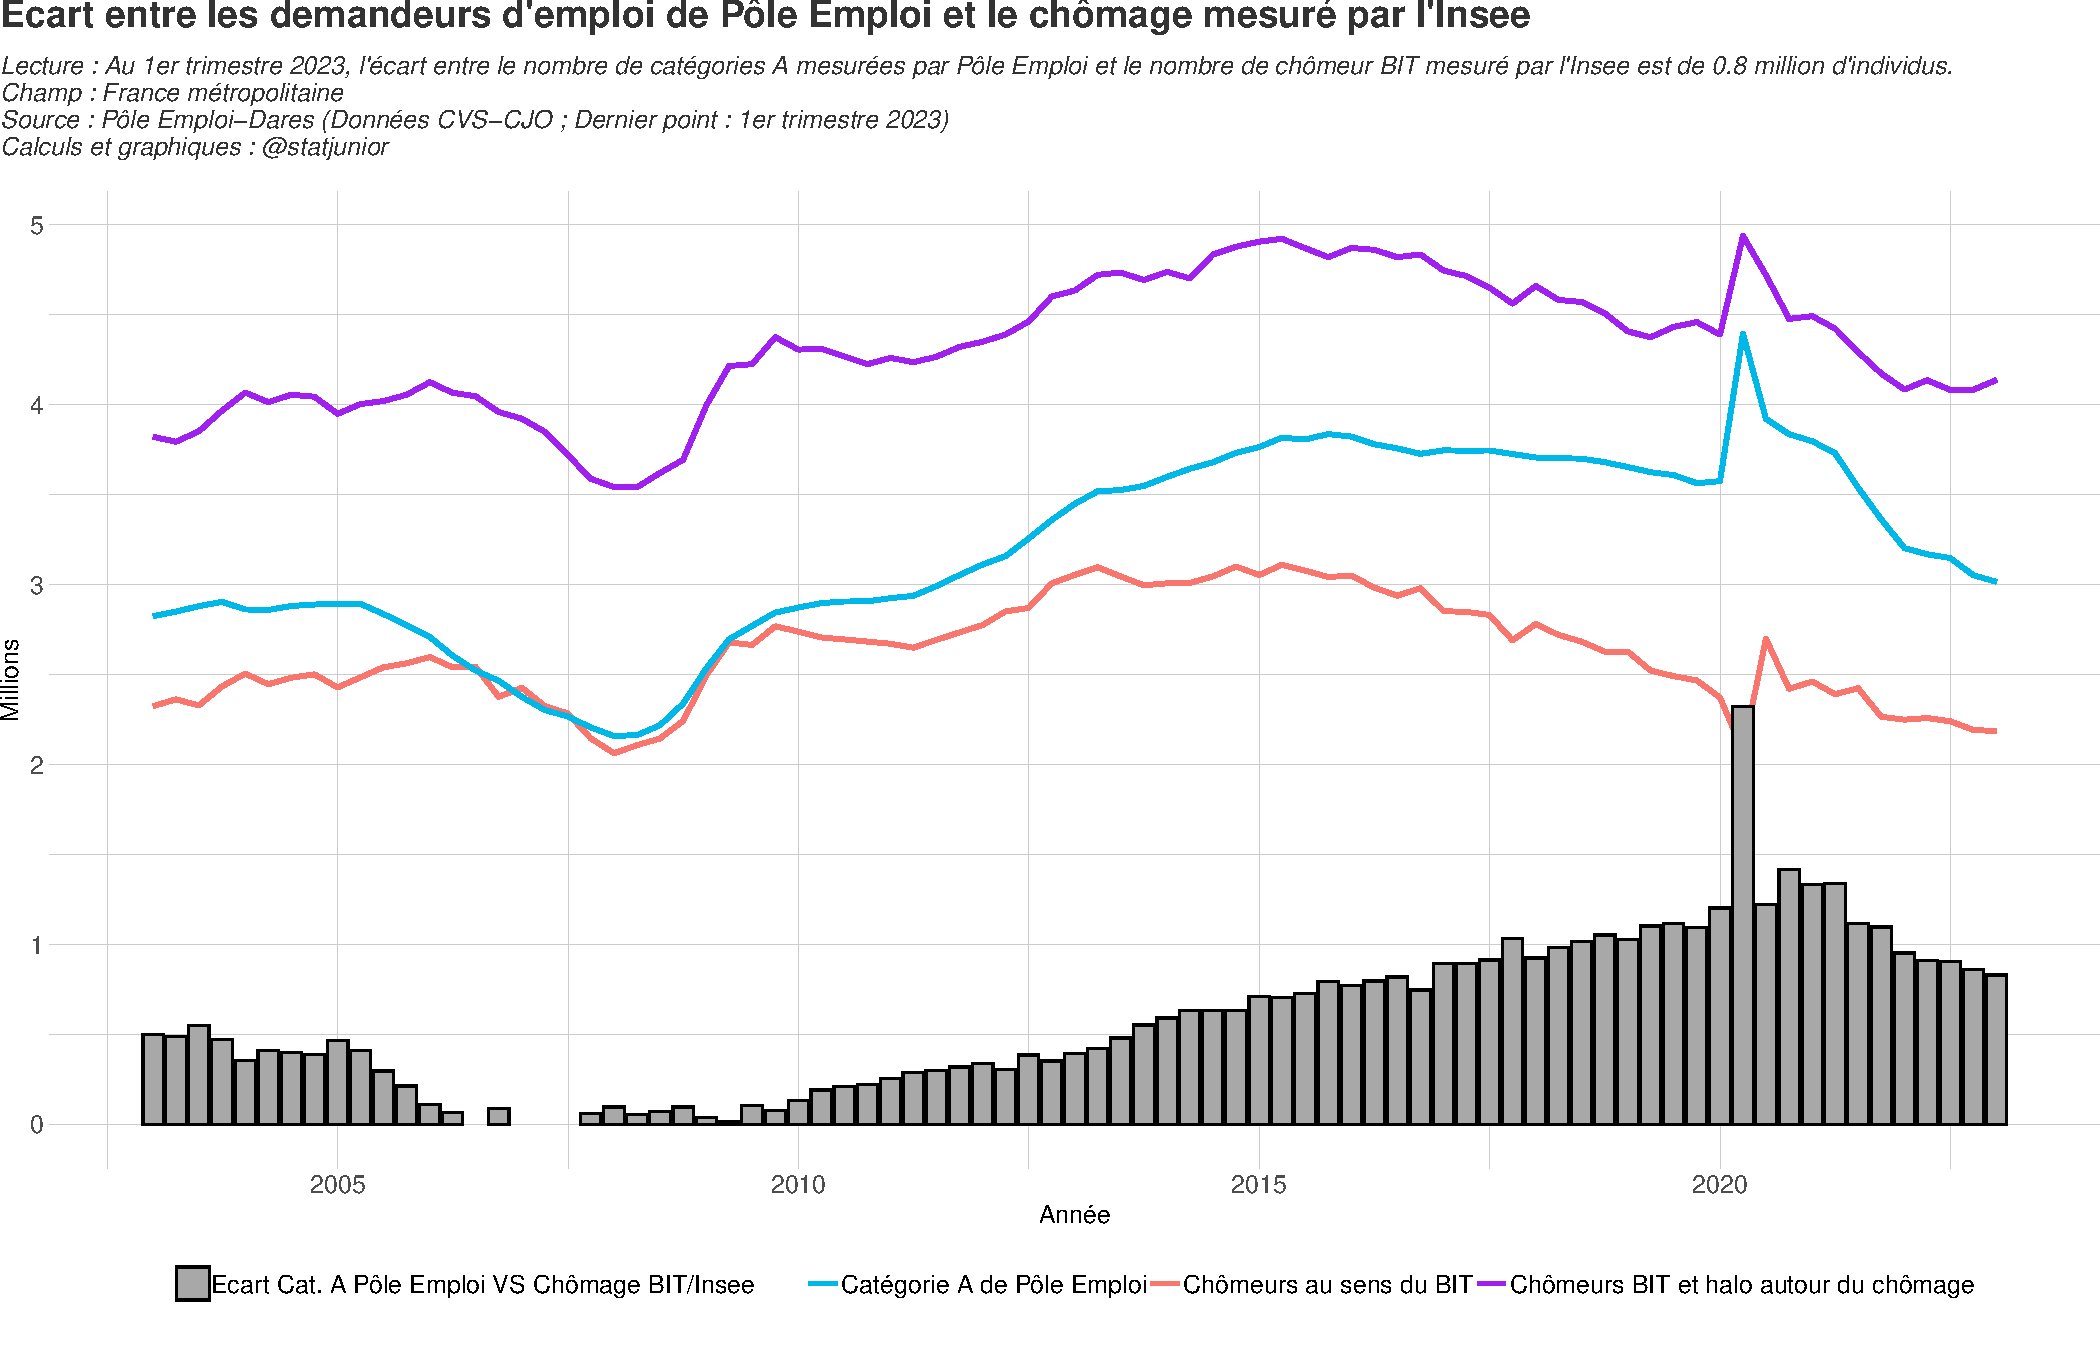
\includegraphics[keepaspectratio]{rapport_pdf_demandeurs_emploi_pole_emploi_files/figure-latex/unnamed-chunk-21-1.pdf}}

\end{document}
